\documentclass[twoside]{book}

% Packages required by doxygen
\usepackage{fixltx2e}
\usepackage{calc}
\usepackage{doxygen}
\usepackage[export]{adjustbox} % also loads graphicx
\usepackage{graphicx}
\usepackage[utf8]{inputenc}
\usepackage{makeidx}
\usepackage{multicol}
\usepackage{multirow}
\PassOptionsToPackage{warn}{textcomp}
\usepackage{textcomp}
\usepackage[nointegrals]{wasysym}
\usepackage[table]{xcolor}

% Font selection
\usepackage[T1]{fontenc}
\usepackage[scaled=.90]{helvet}
\usepackage{courier}
\usepackage{amssymb}
\usepackage{sectsty}
\renewcommand{\familydefault}{\sfdefault}
\allsectionsfont{%
  \fontseries{bc}\selectfont%
  \color{darkgray}%
}
\renewcommand{\DoxyLabelFont}{%
  \fontseries{bc}\selectfont%
  \color{darkgray}%
}
\newcommand{\+}{\discretionary{\mbox{\scriptsize$\hookleftarrow$}}{}{}}

% Page & text layout
\usepackage{geometry}
\geometry{%
  a4paper,%
  top=2.5cm,%
  bottom=2.5cm,%
  left=2.5cm,%
  right=2.5cm%
}
\tolerance=750
\hfuzz=15pt
\hbadness=750
\setlength{\emergencystretch}{15pt}
\setlength{\parindent}{0cm}
\setlength{\parskip}{3ex plus 2ex minus 2ex}
\makeatletter
\renewcommand{\paragraph}{%
  \@startsection{paragraph}{4}{0ex}{-1.0ex}{1.0ex}{%
    \normalfont\normalsize\bfseries\SS@parafont%
  }%
}
\renewcommand{\subparagraph}{%
  \@startsection{subparagraph}{5}{0ex}{-1.0ex}{1.0ex}{%
    \normalfont\normalsize\bfseries\SS@subparafont%
  }%
}
\makeatother

% Headers & footers
\usepackage{fancyhdr}
\pagestyle{fancyplain}
\fancyhead[LE]{\fancyplain{}{\bfseries\thepage}}
\fancyhead[CE]{\fancyplain{}{}}
\fancyhead[RE]{\fancyplain{}{\bfseries\leftmark}}
\fancyhead[LO]{\fancyplain{}{\bfseries\rightmark}}
\fancyhead[CO]{\fancyplain{}{}}
\fancyhead[RO]{\fancyplain{}{\bfseries\thepage}}
\fancyfoot[LE]{\fancyplain{}{}}
\fancyfoot[CE]{\fancyplain{}{}}
\fancyfoot[RE]{\fancyplain{}{\bfseries\scriptsize Generated by Doxygen }}
\fancyfoot[LO]{\fancyplain{}{\bfseries\scriptsize Generated by Doxygen }}
\fancyfoot[CO]{\fancyplain{}{}}
\fancyfoot[RO]{\fancyplain{}{}}
\renewcommand{\footrulewidth}{0.4pt}
\renewcommand{\chaptermark}[1]{%
  \markboth{#1}{}%
}
\renewcommand{\sectionmark}[1]{%
  \markright{\thesection\ #1}%
}

% Indices & bibliography
\usepackage{natbib}
\usepackage[titles]{tocloft}
\setcounter{tocdepth}{3}
\setcounter{secnumdepth}{5}
\makeindex

% Hyperlinks (required, but should be loaded last)
\usepackage{ifpdf}
\ifpdf
  \usepackage[pdftex,pagebackref=true]{hyperref}
\else
  \usepackage[ps2pdf,pagebackref=true]{hyperref}
\fi
\hypersetup{%
  colorlinks=true,%
  linkcolor=blue,%
  citecolor=blue,%
  unicode%
}

% Custom commands
\newcommand{\clearemptydoublepage}{%
  \newpage{\pagestyle{empty}\cleardoublepage}%
}

\usepackage{caption}
\captionsetup{labelsep=space,justification=centering,font={bf},singlelinecheck=off,skip=4pt,position=top}

%===== C O N T E N T S =====

\begin{document}

% Titlepage & ToC
\hypersetup{pageanchor=false,
             bookmarksnumbered=true,
             pdfencoding=unicode
            }
\pagenumbering{roman}
\begin{titlepage}
\vspace*{7cm}
\begin{center}%
{\Large L\+P\+C\+X1102\+\_\+\+C\+M\+S\+I\+S2\+\_\+\+S\+Y\+S\+T\+I\+CK \\[1ex]\large 1.\+0 }\\
\vspace*{1cm}
{\large Generated by Doxygen 1.8.11}\\
\end{center}
\end{titlepage}
\clearemptydoublepage
\tableofcontents
\clearemptydoublepage
\pagenumbering{arabic}
\hypersetup{pageanchor=true}

%--- Begin generated contents ---
\chapter{L\+P\+C\+X1102\+\_\+cmsis2\+\_\+systick}
\label{index}\hypertarget{index}{}Definiciones de C\+M\+S\+IS asociadas al microcontrolador L\+P\+C1102\+This documentation describes the C\+M\+S\+IS Cortex-\/M Core Peripheral Access Layer. It consists of\+:


\begin{DoxyItemize}
\item Cortex-\/M Core Register Definitions
\item Cortex-\/M functions
\item Cortex-\/M instructions
\end{DoxyItemize}

The C\+M\+S\+IS Cortex-\/\+M0 Core Peripheral Access Layer contains C and assembly functions that ease access to the Cortex-\/M Core

Modificaciones C\+I\+T\+E\+D\+EF 2017\+: \begin{DoxyVerb}  - Se agregaron los archivos LPC1102_IOCON.c y .h, que contienen las asociaciones de
    los nombres de los pines en el formato de Puerto y Pin al formato de Fila y columna
    de la matriz de pines BGA. Por ejemplo, el pin P0.8 se traduce en el pin A2.
  - También se incluyeron definiciones de mascaras, bits, funciones, etc.\end{DoxyVerb}
 
\chapter{File Index}
\section{File List}
Here is a list of all files with brief descriptions\+:\begin{DoxyCompactList}
\item\contentsline{section}{/home/telemetria/git/workspaces/tinoc2\+\_\+firmware\+\_\+freertos/\+R\+T\+O\+S\+Demo/\+Source/\hyperlink{cr__startup__lpc11_8c}{cr\+\_\+startup\+\_\+lpc11.\+c} }{\pageref{cr__startup__lpc11_8c}}{}
\item\contentsline{section}{/home/telemetria/git/workspaces/tinoc2\+\_\+firmware\+\_\+freertos/\+R\+T\+O\+S\+Demo/\+Source/\hyperlink{_free_r_t_o_s_config_8h}{Free\+R\+T\+O\+S\+Config.\+h} }{\pageref{_free_r_t_o_s_config_8h}}{}
\item\contentsline{section}{/home/telemetria/git/workspaces/tinoc2\+\_\+firmware\+\_\+freertos/\+R\+T\+O\+S\+Demo/\+Source/\hyperlink{_int_queue_timer_8c}{Int\+Queue\+Timer.\+c} }{\pageref{_int_queue_timer_8c}}{}
\item\contentsline{section}{/home/telemetria/git/workspaces/tinoc2\+\_\+firmware\+\_\+freertos/\+R\+T\+O\+S\+Demo/\+Source/\hyperlink{_int_queue_timer_8h}{Int\+Queue\+Timer.\+h} }{\pageref{_int_queue_timer_8h}}{}
\item\contentsline{section}{/home/telemetria/git/workspaces/tinoc2\+\_\+firmware\+\_\+freertos/\+R\+T\+O\+S\+Demo/\+Source/\hyperlink{main-blinky_8c}{main-\/blinky.\+c} }{\pageref{main-blinky_8c}}{}
\item\contentsline{section}{/home/telemetria/git/workspaces/tinoc2\+\_\+firmware\+\_\+freertos/\+R\+T\+O\+S\+Demo/\+Source/\hyperlink{main-full_8c}{main-\/full.\+c} }{\pageref{main-full_8c}}{}
\item\contentsline{section}{/home/telemetria/git/workspaces/tinoc2\+\_\+firmware\+\_\+freertos/\+R\+T\+O\+S\+Demo/\+Source/\hyperlink{main_8c}{main.\+c} \\*Archivo principal del proyecto }{\pageref{main_8c}}{}
\item\contentsline{section}{/home/telemetria/git/workspaces/tinoc2\+\_\+firmware\+\_\+freertos/\+R\+T\+O\+S\+Demo/\+Source/\hyperlink{_reg_test_8c}{Reg\+Test.\+c} }{\pageref{_reg_test_8c}}{}
\item\contentsline{section}{/home/telemetria/git/workspaces/tinoc2\+\_\+firmware\+\_\+freertos/\+R\+T\+O\+S\+Demo/\+Source/\+Common\+\_\+\+Demo\+\_\+\+Tasks/\hyperlink{blocktim_8c}{blocktim.\+c} }{\pageref{blocktim_8c}}{}
\item\contentsline{section}{/home/telemetria/git/workspaces/tinoc2\+\_\+firmware\+\_\+freertos/\+R\+T\+O\+S\+Demo/\+Source/\+Common\+\_\+\+Demo\+\_\+\+Tasks/\hyperlink{countsem_8c}{countsem.\+c} }{\pageref{countsem_8c}}{}
\item\contentsline{section}{/home/telemetria/git/workspaces/tinoc2\+\_\+firmware\+\_\+freertos/\+R\+T\+O\+S\+Demo/\+Source/\+Common\+\_\+\+Demo\+\_\+\+Tasks/\hyperlink{_int_queue_8c}{Int\+Queue.\+c} }{\pageref{_int_queue_8c}}{}
\item\contentsline{section}{/home/telemetria/git/workspaces/tinoc2\+\_\+firmware\+\_\+freertos/\+R\+T\+O\+S\+Demo/\+Source/\+Common\+\_\+\+Demo\+\_\+\+Tasks/\hyperlink{recmutex_8c}{recmutex.\+c} }{\pageref{recmutex_8c}}{}
\item\contentsline{section}{/home/telemetria/git/workspaces/tinoc2\+\_\+firmware\+\_\+freertos/\+R\+T\+O\+S\+Demo/\+Source/\+Common\+\_\+\+Demo\+\_\+\+Tasks/include/\hyperlink{blocktim_8h}{blocktim.\+h} }{\pageref{blocktim_8h}}{}
\item\contentsline{section}{/home/telemetria/git/workspaces/tinoc2\+\_\+firmware\+\_\+freertos/\+R\+T\+O\+S\+Demo/\+Source/\+Common\+\_\+\+Demo\+\_\+\+Tasks/include/\hyperlink{countsem_8h}{countsem.\+h} }{\pageref{countsem_8h}}{}
\item\contentsline{section}{/home/telemetria/git/workspaces/tinoc2\+\_\+firmware\+\_\+freertos/\+R\+T\+O\+S\+Demo/\+Source/\+Common\+\_\+\+Demo\+\_\+\+Tasks/include/\hyperlink{_int_queue_8h}{Int\+Queue.\+h} }{\pageref{_int_queue_8h}}{}
\item\contentsline{section}{/home/telemetria/git/workspaces/tinoc2\+\_\+firmware\+\_\+freertos/\+R\+T\+O\+S\+Demo/\+Source/\+Common\+\_\+\+Demo\+\_\+\+Tasks/include/\hyperlink{recmutex_8h}{recmutex.\+h} }{\pageref{recmutex_8h}}{}
\item\contentsline{section}{/home/telemetria/git/workspaces/tinoc2\+\_\+firmware\+\_\+freertos/\+R\+T\+O\+S\+Demo/\+Source/flash/\hyperlink{flash_8c}{flash.\+c} \\*Funciones de manejo de memoria flash }{\pageref{flash_8c}}{}
\item\contentsline{section}{/home/telemetria/git/workspaces/tinoc2\+\_\+firmware\+\_\+freertos/\+R\+T\+O\+S\+Demo/\+Source/flash/\hyperlink{flash_8h}{flash.\+h} \\*Header de \hyperlink{flash_8c}{flash.\+c} }{\pageref{flash_8h}}{}
\item\contentsline{section}{/home/telemetria/git/workspaces/tinoc2\+\_\+firmware\+\_\+freertos/\+R\+T\+O\+S\+Demo/\+Source/\+Free\+R\+T\+O\+S\+\_\+\+Source/\hyperlink{list_8c}{list.\+c} }{\pageref{list_8c}}{}
\item\contentsline{section}{/home/telemetria/git/workspaces/tinoc2\+\_\+firmware\+\_\+freertos/\+R\+T\+O\+S\+Demo/\+Source/\+Free\+R\+T\+O\+S\+\_\+\+Source/\hyperlink{queue_8c}{queue.\+c} }{\pageref{queue_8c}}{}
\item\contentsline{section}{/home/telemetria/git/workspaces/tinoc2\+\_\+firmware\+\_\+freertos/\+R\+T\+O\+S\+Demo/\+Source/\+Free\+R\+T\+O\+S\+\_\+\+Source/\hyperlink{tasks_8c}{tasks.\+c} }{\pageref{tasks_8c}}{}
\item\contentsline{section}{/home/telemetria/git/workspaces/tinoc2\+\_\+firmware\+\_\+freertos/\+R\+T\+O\+S\+Demo/\+Source/\+Free\+R\+T\+O\+S\+\_\+\+Source/\hyperlink{timers_8c}{timers.\+c} }{\pageref{timers_8c}}{}
\item\contentsline{section}{/home/telemetria/git/workspaces/tinoc2\+\_\+firmware\+\_\+freertos/\+R\+T\+O\+S\+Demo/\+Source/\+Free\+R\+T\+O\+S\+\_\+\+Source/include/\hyperlink{croutine_8h}{croutine.\+h} }{\pageref{croutine_8h}}{}
\item\contentsline{section}{/home/telemetria/git/workspaces/tinoc2\+\_\+firmware\+\_\+freertos/\+R\+T\+O\+S\+Demo/\+Source/\+Free\+R\+T\+O\+S\+\_\+\+Source/include/\hyperlink{deprecated__definitions_8h}{deprecated\+\_\+definitions.\+h} }{\pageref{deprecated__definitions_8h}}{}
\item\contentsline{section}{/home/telemetria/git/workspaces/tinoc2\+\_\+firmware\+\_\+freertos/\+R\+T\+O\+S\+Demo/\+Source/\+Free\+R\+T\+O\+S\+\_\+\+Source/include/\hyperlink{event__groups_8h}{event\+\_\+groups.\+h} }{\pageref{event__groups_8h}}{}
\item\contentsline{section}{/home/telemetria/git/workspaces/tinoc2\+\_\+firmware\+\_\+freertos/\+R\+T\+O\+S\+Demo/\+Source/\+Free\+R\+T\+O\+S\+\_\+\+Source/include/\hyperlink{_free_r_t_o_s_8h}{Free\+R\+T\+O\+S.\+h} }{\pageref{_free_r_t_o_s_8h}}{}
\item\contentsline{section}{/home/telemetria/git/workspaces/tinoc2\+\_\+firmware\+\_\+freertos/\+R\+T\+O\+S\+Demo/\+Source/\+Free\+R\+T\+O\+S\+\_\+\+Source/include/\hyperlink{list_8h}{list.\+h} }{\pageref{list_8h}}{}
\item\contentsline{section}{/home/telemetria/git/workspaces/tinoc2\+\_\+firmware\+\_\+freertos/\+R\+T\+O\+S\+Demo/\+Source/\+Free\+R\+T\+O\+S\+\_\+\+Source/include/\hyperlink{mpu__prototypes_8h}{mpu\+\_\+prototypes.\+h} }{\pageref{mpu__prototypes_8h}}{}
\item\contentsline{section}{/home/telemetria/git/workspaces/tinoc2\+\_\+firmware\+\_\+freertos/\+R\+T\+O\+S\+Demo/\+Source/\+Free\+R\+T\+O\+S\+\_\+\+Source/include/\hyperlink{mpu__wrappers_8h}{mpu\+\_\+wrappers.\+h} }{\pageref{mpu__wrappers_8h}}{}
\item\contentsline{section}{/home/telemetria/git/workspaces/tinoc2\+\_\+firmware\+\_\+freertos/\+R\+T\+O\+S\+Demo/\+Source/\+Free\+R\+T\+O\+S\+\_\+\+Source/include/\hyperlink{portable_8h}{portable.\+h} }{\pageref{portable_8h}}{}
\item\contentsline{section}{/home/telemetria/git/workspaces/tinoc2\+\_\+firmware\+\_\+freertos/\+R\+T\+O\+S\+Demo/\+Source/\+Free\+R\+T\+O\+S\+\_\+\+Source/include/\hyperlink{projdefs_8h}{projdefs.\+h} }{\pageref{projdefs_8h}}{}
\item\contentsline{section}{/home/telemetria/git/workspaces/tinoc2\+\_\+firmware\+\_\+freertos/\+R\+T\+O\+S\+Demo/\+Source/\+Free\+R\+T\+O\+S\+\_\+\+Source/include/\hyperlink{queue_8h}{queue.\+h} }{\pageref{queue_8h}}{}
\item\contentsline{section}{/home/telemetria/git/workspaces/tinoc2\+\_\+firmware\+\_\+freertos/\+R\+T\+O\+S\+Demo/\+Source/\+Free\+R\+T\+O\+S\+\_\+\+Source/include/\hyperlink{semphr_8h}{semphr.\+h} }{\pageref{semphr_8h}}{}
\item\contentsline{section}{/home/telemetria/git/workspaces/tinoc2\+\_\+firmware\+\_\+freertos/\+R\+T\+O\+S\+Demo/\+Source/\+Free\+R\+T\+O\+S\+\_\+\+Source/include/\hyperlink{_stack_macros_8h}{Stack\+Macros.\+h} }{\pageref{_stack_macros_8h}}{}
\item\contentsline{section}{/home/telemetria/git/workspaces/tinoc2\+\_\+firmware\+\_\+freertos/\+R\+T\+O\+S\+Demo/\+Source/\+Free\+R\+T\+O\+S\+\_\+\+Source/include/\hyperlink{task_8h}{task.\+h} }{\pageref{task_8h}}{}
\item\contentsline{section}{/home/telemetria/git/workspaces/tinoc2\+\_\+firmware\+\_\+freertos/\+R\+T\+O\+S\+Demo/\+Source/\+Free\+R\+T\+O\+S\+\_\+\+Source/include/\hyperlink{timers_8h}{timers.\+h} }{\pageref{timers_8h}}{}
\item\contentsline{section}{/home/telemetria/git/workspaces/tinoc2\+\_\+firmware\+\_\+freertos/\+R\+T\+O\+S\+Demo/\+Source/\+Free\+R\+T\+O\+S\+\_\+\+Source/portable/\+G\+C\+C/\+A\+R\+M\+\_\+\+C\+M0/\hyperlink{port_8c}{port.\+c} }{\pageref{port_8c}}{}
\item\contentsline{section}{/home/telemetria/git/workspaces/tinoc2\+\_\+firmware\+\_\+freertos/\+R\+T\+O\+S\+Demo/\+Source/\+Free\+R\+T\+O\+S\+\_\+\+Source/portable/\+G\+C\+C/\+A\+R\+M\+\_\+\+C\+M0/\hyperlink{portmacro_8h}{portmacro.\+h} }{\pageref{portmacro_8h}}{}
\item\contentsline{section}{/home/telemetria/git/workspaces/tinoc2\+\_\+firmware\+\_\+freertos/\+R\+T\+O\+S\+Demo/\+Source/\+Free\+R\+T\+O\+S\+\_\+\+Source/portable/\+Mem\+Mang/\hyperlink{heap__1_8c}{heap\+\_\+1.\+c} }{\pageref{heap__1_8c}}{}
\item\contentsline{section}{/home/telemetria/git/workspaces/tinoc2\+\_\+firmware\+\_\+freertos/\+R\+T\+O\+S\+Demo/\+Source/gpio/\hyperlink{gpio_8c}{gpio.\+c} \\*G\+P\+IO C file for N\+XP L\+P\+C11xx Family Microprocessors }{\pageref{gpio_8c}}{}
\item\contentsline{section}{/home/telemetria/git/workspaces/tinoc2\+\_\+firmware\+\_\+freertos/\+R\+T\+O\+S\+Demo/\+Source/gpio/\hyperlink{gpio_8h}{gpio.\+h} }{\pageref{gpio_8h}}{}
\item\contentsline{section}{/home/telemetria/git/workspaces/tinoc2\+\_\+firmware\+\_\+freertos/\+R\+T\+O\+S\+Demo/\+Source/hardware/\hyperlink{hardware__aplicacion_8c}{hardware\+\_\+aplicacion.\+c} \\*Funciones de inicialización del hardware específicas para la aplicacion }{\pageref{hardware__aplicacion_8c}}{}
\item\contentsline{section}{/home/telemetria/git/workspaces/tinoc2\+\_\+firmware\+\_\+freertos/\+R\+T\+O\+S\+Demo/\+Source/hardware/\hyperlink{hardware__aplicacion_8h}{hardware\+\_\+aplicacion.\+h} \\*Header del archivo \hyperlink{hardware__aplicacion_8h}{hardware\+\_\+aplicacion.\+h} }{\pageref{hardware__aplicacion_8h}}{}
\item\contentsline{section}{/home/telemetria/git/workspaces/tinoc2\+\_\+firmware\+\_\+freertos/\+R\+T\+O\+S\+Demo/\+Source/hardware/\hyperlink{tinoc__lpclink_8c}{tinoc\+\_\+lpclink.\+c} \\*Funciones de inicialización del hardware específicas para la placa T\+I\+N\+O\+C\+\_\+\+L\+P\+C\+L\+I\+NK }{\pageref{tinoc__lpclink_8c}}{}
\item\contentsline{section}{/home/telemetria/git/workspaces/tinoc2\+\_\+firmware\+\_\+freertos/\+R\+T\+O\+S\+Demo/\+Source/hardware/\hyperlink{tinoc__lpclink_8h}{tinoc\+\_\+lpclink.\+h} \\*Header del archivo \hyperlink{tinoc__lpclink_8c}{tinoc\+\_\+lpclink.\+c} }{\pageref{tinoc__lpclink_8h}}{}
\item\contentsline{section}{/home/telemetria/git/workspaces/tinoc2\+\_\+firmware\+\_\+freertos/\+R\+T\+O\+S\+Demo/\+Source/leds/\hyperlink{leds_8c}{leds.\+c} \\*Funciones de manejo de leds específicas para la aplicacion }{\pageref{leds_8c}}{}
\item\contentsline{section}{/home/telemetria/git/workspaces/tinoc2\+\_\+firmware\+\_\+freertos/\+R\+T\+O\+S\+Demo/\+Source/leds/\hyperlink{leds_8h}{leds.\+h} \\*Header del archivo \hyperlink{leds_8c}{leds.\+c} }{\pageref{leds_8h}}{}
\item\contentsline{section}{/home/telemetria/git/workspaces/tinoc2\+\_\+firmware\+\_\+freertos/\+R\+T\+O\+S\+Demo/\+Source/\+U\+A\+R\+T/\hyperlink{colas_8c}{colas.\+c} \\*Funciones relacionadas con el manejo de colas }{\pageref{colas_8c}}{}
\item\contentsline{section}{/home/telemetria/git/workspaces/tinoc2\+\_\+firmware\+\_\+freertos/\+R\+T\+O\+S\+Demo/\+Source/\+U\+A\+R\+T/\hyperlink{colas_8h}{colas.\+h} \\*Header del archivo \char`\"{}colas.\+c\char`\"{} }{\pageref{colas_8h}}{}
\item\contentsline{section}{/home/telemetria/git/workspaces/tinoc2\+\_\+firmware\+\_\+freertos/\+R\+T\+O\+S\+Demo/\+Source/\+U\+A\+R\+T/\hyperlink{uart_8c}{uart.\+c} \\*U\+A\+RT A\+PI file for N\+XP L\+P\+C11xx Family Microprocessors~\newline
 Archivo modificado para trabajar como driver dentro del~\newline
 protocolo de comunicacion P\+C\+P1~\newline
~\newline
 {\bfseries History} }{\pageref{uart_8c}}{}
\item\contentsline{section}{/home/telemetria/git/workspaces/tinoc2\+\_\+firmware\+\_\+freertos/\+R\+T\+O\+S\+Demo/\+Source/\+U\+A\+R\+T/\hyperlink{uart_8h}{uart.\+h} \\*Header del archivo \hyperlink{uart_8c}{uart.\+c} }{\pageref{uart_8h}}{}
\end{DoxyCompactList}

\chapter{File Documentation}
\hypertarget{cr__startup__lpc1102_8d}{}\section{/home/piro8/\+Documentos/\+T\+I\+N\+O\+C2/\+T\+I\+N\+O\+C2\+\_\+\+F\+I\+R\+M\+W\+A\+R\+E\+\_\+\+F\+R\+E\+E\+R\+T\+O\+S/\+L\+P\+C\+X1102\+\_\+cmsis2\+\_\+systick/\+Debug/src/cr\+\_\+startup\+\_\+lpc1102.d File Reference}
\label{cr__startup__lpc1102_8d}\index{/home/piro8/\+Documentos/\+T\+I\+N\+O\+C2/\+T\+I\+N\+O\+C2\+\_\+\+F\+I\+R\+M\+W\+A\+R\+E\+\_\+\+F\+R\+E\+E\+R\+T\+O\+S/\+L\+P\+C\+X1102\+\_\+cmsis2\+\_\+systick/\+Debug/src/cr\+\_\+startup\+\_\+lpc1102.\+d@{/home/piro8/\+Documentos/\+T\+I\+N\+O\+C2/\+T\+I\+N\+O\+C2\+\_\+\+F\+I\+R\+M\+W\+A\+R\+E\+\_\+\+F\+R\+E\+E\+R\+T\+O\+S/\+L\+P\+C\+X1102\+\_\+cmsis2\+\_\+systick/\+Debug/src/cr\+\_\+startup\+\_\+lpc1102.\+d}}

\hypertarget{gpio_8d}{}\section{/home/piro8/\+Documentos/\+T\+I\+N\+O\+C2/\+T\+I\+N\+O\+C2\+\_\+\+F\+I\+R\+M\+W\+A\+R\+E\+\_\+\+F\+R\+E\+E\+R\+T\+O\+S/\+L\+P\+C\+X1102\+\_\+cmsis2\+\_\+systick/\+Debug/src/gpio.d File Reference}
\label{gpio_8d}\index{/home/piro8/\+Documentos/\+T\+I\+N\+O\+C2/\+T\+I\+N\+O\+C2\+\_\+\+F\+I\+R\+M\+W\+A\+R\+E\+\_\+\+F\+R\+E\+E\+R\+T\+O\+S/\+L\+P\+C\+X1102\+\_\+cmsis2\+\_\+systick/\+Debug/src/gpio.\+d@{/home/piro8/\+Documentos/\+T\+I\+N\+O\+C2/\+T\+I\+N\+O\+C2\+\_\+\+F\+I\+R\+M\+W\+A\+R\+E\+\_\+\+F\+R\+E\+E\+R\+T\+O\+S/\+L\+P\+C\+X1102\+\_\+cmsis2\+\_\+systick/\+Debug/src/gpio.\+d}}

\hypertarget{lpc1102__isp_8d}{}\section{/home/piro8/\+Documentos/\+T\+I\+N\+O\+C2/\+T\+I\+N\+O\+C2\+\_\+\+F\+I\+R\+M\+W\+A\+R\+E\+\_\+\+F\+R\+E\+E\+R\+T\+O\+S/\+L\+P\+C\+X1102\+\_\+cmsis2\+\_\+systick/\+Debug/src/lpc1102\+\_\+isp.d File Reference}
\label{lpc1102__isp_8d}\index{/home/piro8/\+Documentos/\+T\+I\+N\+O\+C2/\+T\+I\+N\+O\+C2\+\_\+\+F\+I\+R\+M\+W\+A\+R\+E\+\_\+\+F\+R\+E\+E\+R\+T\+O\+S/\+L\+P\+C\+X1102\+\_\+cmsis2\+\_\+systick/\+Debug/src/lpc1102\+\_\+isp.\+d@{/home/piro8/\+Documentos/\+T\+I\+N\+O\+C2/\+T\+I\+N\+O\+C2\+\_\+\+F\+I\+R\+M\+W\+A\+R\+E\+\_\+\+F\+R\+E\+E\+R\+T\+O\+S/\+L\+P\+C\+X1102\+\_\+cmsis2\+\_\+systick/\+Debug/src/lpc1102\+\_\+isp.\+d}}

\hypertarget{systick_8d}{}\section{/home/piro8/\+Documentos/\+T\+I\+N\+O\+C2/\+T\+I\+N\+O\+C2\+\_\+\+F\+I\+R\+M\+W\+A\+R\+E\+\_\+\+F\+R\+E\+E\+R\+T\+O\+S/\+L\+P\+C\+X1102\+\_\+cmsis2\+\_\+systick/\+Debug/src/systick.d File Reference}
\label{systick_8d}\index{/home/piro8/\+Documentos/\+T\+I\+N\+O\+C2/\+T\+I\+N\+O\+C2\+\_\+\+F\+I\+R\+M\+W\+A\+R\+E\+\_\+\+F\+R\+E\+E\+R\+T\+O\+S/\+L\+P\+C\+X1102\+\_\+cmsis2\+\_\+systick/\+Debug/src/systick.\+d@{/home/piro8/\+Documentos/\+T\+I\+N\+O\+C2/\+T\+I\+N\+O\+C2\+\_\+\+F\+I\+R\+M\+W\+A\+R\+E\+\_\+\+F\+R\+E\+E\+R\+T\+O\+S/\+L\+P\+C\+X1102\+\_\+cmsis2\+\_\+systick/\+Debug/src/systick.\+d}}

\hypertarget{cr__startup__lpc1102_8c}{}\section{/home/piro8/\+Documentos/\+T\+I\+N\+O\+C2/\+T\+I\+N\+O\+C2\+\_\+\+F\+I\+R\+M\+W\+A\+R\+E\+\_\+\+F\+R\+E\+E\+R\+T\+O\+S/\+L\+P\+C\+X1102\+\_\+cmsis2\+\_\+systick/src/cr\+\_\+startup\+\_\+lpc1102.c File Reference}
\label{cr__startup__lpc1102_8c}\index{/home/piro8/\+Documentos/\+T\+I\+N\+O\+C2/\+T\+I\+N\+O\+C2\+\_\+\+F\+I\+R\+M\+W\+A\+R\+E\+\_\+\+F\+R\+E\+E\+R\+T\+O\+S/\+L\+P\+C\+X1102\+\_\+cmsis2\+\_\+systick/src/cr\+\_\+startup\+\_\+lpc1102.\+c@{/home/piro8/\+Documentos/\+T\+I\+N\+O\+C2/\+T\+I\+N\+O\+C2\+\_\+\+F\+I\+R\+M\+W\+A\+R\+E\+\_\+\+F\+R\+E\+E\+R\+T\+O\+S/\+L\+P\+C\+X1102\+\_\+cmsis2\+\_\+systick/src/cr\+\_\+startup\+\_\+lpc1102.\+c}}
\subsection*{Macros}
\begin{DoxyCompactItemize}
\item 
\#define \hyperlink{cr__startup__lpc1102_8c_ad1480e9557edcc543498ca259cee6c7d}{W\+E\+AK}~\hyperlink{cr__startup__lpc1102_8c_adce420b900676fa0caed5a713cac82fb}{\+\_\+\+\_\+attribute\+\_\+\+\_\+} ((weak))
\item 
\#define \hyperlink{cr__startup__lpc1102_8c_a0bcadbfb9fcd175b07b4d0463e54397f}{A\+L\+I\+AS}(f)~\hyperlink{cr__startup__lpc1102_8c_adce420b900676fa0caed5a713cac82fb}{\+\_\+\+\_\+attribute\+\_\+\+\_\+} ((weak, alias (\#f)))
\end{DoxyCompactItemize}
\subsection*{Functions}
\begin{DoxyCompactItemize}
\item 
void \hyperlink{cr__startup__lpc1102_8c_a516ff8924be921fa3a1bb7754b1f5734}{Reset\+I\+SR} (void)
\item 
\hyperlink{cr__startup__lpc1102_8c_ad1480e9557edcc543498ca259cee6c7d}{W\+E\+AK} void \hyperlink{cr__startup__lpc1102_8c_ae5eb40c717803d8eae9630d1f7237fd7}{N\+M\+I\+\_\+\+Handler} (void)
\item 
\hyperlink{cr__startup__lpc1102_8c_ad1480e9557edcc543498ca259cee6c7d}{W\+E\+AK} void \hyperlink{cr__startup__lpc1102_8c_abf5d8b089d5aceaf6a281f9bb81ac731}{Hard\+Fault\+\_\+\+Handler} (void)
\item 
\hyperlink{cr__startup__lpc1102_8c_ad1480e9557edcc543498ca259cee6c7d}{W\+E\+AK} void \hyperlink{cr__startup__lpc1102_8c_a553d3c6fbc0ff764fa70b866b5c79e3e}{S\+V\+C\+\_\+\+Handler} (void)
\item 
\hyperlink{cr__startup__lpc1102_8c_ad1480e9557edcc543498ca259cee6c7d}{W\+E\+AK} void \hyperlink{cr__startup__lpc1102_8c_a24fd4a50e601121b29d900129e4602db}{Pend\+S\+V\+\_\+\+Handler} (void)
\item 
\hyperlink{cr__startup__lpc1102_8c_ad1480e9557edcc543498ca259cee6c7d}{W\+E\+AK} void \hyperlink{cr__startup__lpc1102_8c_ab80f32111a0725c9f4cdfb9d6c9b7f82}{Sys\+Tick\+\_\+\+Handler} (void)
\item 
\hyperlink{cr__startup__lpc1102_8c_ad1480e9557edcc543498ca259cee6c7d}{W\+E\+AK} void \hyperlink{cr__startup__lpc1102_8c_abf37bc77b79673bf5babd3ac42291616}{Int\+Default\+Handler} (void)
\item 
void \hyperlink{cr__startup__lpc1102_8c_a052da4fb18ef06d91b58d3c786e44fea}{C\+A\+N\+\_\+\+I\+R\+Q\+Handler} (void S\+S\+P1\+\_\+\+I\+R\+Q\+Handler() \hyperlink{cr__startup__lpc1102_8c_a0bcadbfb9fcd175b07b4d0463e54397f}{A\+L\+I\+AS}(\hyperlink{cr__startup__lpc1102_8c_abf37bc77b79673bf5babd3ac42291616}{Int\+Default\+Handler}) void)
\item 
\hyperlink{cr__startup__lpc1102_8c_adce420b900676fa0caed5a713cac82fb}{\+\_\+\+\_\+attribute\+\_\+\+\_\+} ((section(\char`\"{}.after\+\_\+vectors\char`\"{})))
\end{DoxyCompactItemize}
\subsection*{Variables}
\begin{DoxyCompactItemize}
\item 
unsigned int \hyperlink{cr__startup__lpc1102_8c_aa8f8f3229652f39c672fdb9309f96247}{\+\_\+\+\_\+data\+\_\+section\+\_\+table}
\item 
unsigned int \hyperlink{cr__startup__lpc1102_8c_a09092262b7b68d7b89c9dcea506c5388}{\+\_\+\+\_\+data\+\_\+section\+\_\+table\+\_\+end}
\item 
unsigned int \hyperlink{cr__startup__lpc1102_8c_a5876e5d2bb28455dd6e109ceb6a328d8}{\+\_\+\+\_\+bss\+\_\+section\+\_\+table}
\item 
unsigned int \hyperlink{cr__startup__lpc1102_8c_a6365f813efb5c531f6eb7f031e28e6c1}{\+\_\+\+\_\+bss\+\_\+section\+\_\+table\+\_\+end}
\end{DoxyCompactItemize}


\subsection{Macro Definition Documentation}
\index{cr\+\_\+startup\+\_\+lpc1102.\+c@{cr\+\_\+startup\+\_\+lpc1102.\+c}!A\+L\+I\+AS@{A\+L\+I\+AS}}
\index{A\+L\+I\+AS@{A\+L\+I\+AS}!cr\+\_\+startup\+\_\+lpc1102.\+c@{cr\+\_\+startup\+\_\+lpc1102.\+c}}
\subsubsection[{\texorpdfstring{A\+L\+I\+AS}{ALIAS}}]{\setlength{\rightskip}{0pt plus 5cm}\#define A\+L\+I\+AS(
\begin{DoxyParamCaption}
\item[{}]{f}
\end{DoxyParamCaption}
)~{\bf \+\_\+\+\_\+attribute\+\_\+\+\_\+} ((weak, alias (\#f)))}\hypertarget{cr__startup__lpc1102_8c_a0bcadbfb9fcd175b07b4d0463e54397f}{}\label{cr__startup__lpc1102_8c_a0bcadbfb9fcd175b07b4d0463e54397f}


Definition at line 46 of file cr\+\_\+startup\+\_\+lpc1102.\+c.

\index{cr\+\_\+startup\+\_\+lpc1102.\+c@{cr\+\_\+startup\+\_\+lpc1102.\+c}!W\+E\+AK@{W\+E\+AK}}
\index{W\+E\+AK@{W\+E\+AK}!cr\+\_\+startup\+\_\+lpc1102.\+c@{cr\+\_\+startup\+\_\+lpc1102.\+c}}
\subsubsection[{\texorpdfstring{W\+E\+AK}{WEAK}}]{\setlength{\rightskip}{0pt plus 5cm}\#define W\+E\+AK~{\bf \+\_\+\+\_\+attribute\+\_\+\+\_\+} ((weak))}\hypertarget{cr__startup__lpc1102_8c_ad1480e9557edcc543498ca259cee6c7d}{}\label{cr__startup__lpc1102_8c_ad1480e9557edcc543498ca259cee6c7d}


Definition at line 45 of file cr\+\_\+startup\+\_\+lpc1102.\+c.



\subsection{Function Documentation}
\index{cr\+\_\+startup\+\_\+lpc1102.\+c@{cr\+\_\+startup\+\_\+lpc1102.\+c}!\+\_\+\+\_\+attribute\+\_\+\+\_\+@{\+\_\+\+\_\+attribute\+\_\+\+\_\+}}
\index{\+\_\+\+\_\+attribute\+\_\+\+\_\+@{\+\_\+\+\_\+attribute\+\_\+\+\_\+}!cr\+\_\+startup\+\_\+lpc1102.\+c@{cr\+\_\+startup\+\_\+lpc1102.\+c}}
\subsubsection[{\texorpdfstring{\+\_\+\+\_\+attribute\+\_\+\+\_\+((section("".\+after\+\_\+vectors"")))}{__attribute__((section(".after_vectors")))}}]{\setlength{\rightskip}{0pt plus 5cm}\+\_\+\+\_\+attribute\+\_\+\+\_\+ (
\begin{DoxyParamCaption}
\item[{(section(\char`\"{}.after\+\_\+vectors\char`\"{}))}]{}
\end{DoxyParamCaption}
)}\hypertarget{cr__startup__lpc1102_8c_adce420b900676fa0caed5a713cac82fb}{}\label{cr__startup__lpc1102_8c_adce420b900676fa0caed5a713cac82fb}


Definition at line 200 of file cr\+\_\+startup\+\_\+lpc1102.\+c.

\index{cr\+\_\+startup\+\_\+lpc1102.\+c@{cr\+\_\+startup\+\_\+lpc1102.\+c}!C\+A\+N\+\_\+\+I\+R\+Q\+Handler@{C\+A\+N\+\_\+\+I\+R\+Q\+Handler}}
\index{C\+A\+N\+\_\+\+I\+R\+Q\+Handler@{C\+A\+N\+\_\+\+I\+R\+Q\+Handler}!cr\+\_\+startup\+\_\+lpc1102.\+c@{cr\+\_\+startup\+\_\+lpc1102.\+c}}
\subsubsection[{\texorpdfstring{C\+A\+N\+\_\+\+I\+R\+Q\+Handler(void S\+S\+P1\+\_\+\+I\+R\+Q\+Handler() A\+L\+I\+A\+S(\+Int\+Default\+Handler) void)}{CAN_IRQHandler(void SSP1_IRQHandler() ALIAS(IntDefaultHandler) void)}}]{\setlength{\rightskip}{0pt plus 5cm}void C\+A\+N\+\_\+\+I\+R\+Q\+Handler (
\begin{DoxyParamCaption}
\item[{void S\+S\+P1\+\_\+\+I\+R\+Q\+Handler () {\bf A\+L\+I\+AS}({\bf Int\+Default\+Handler})}]{void}
\end{DoxyParamCaption}
)}\hypertarget{cr__startup__lpc1102_8c_a052da4fb18ef06d91b58d3c786e44fea}{}\label{cr__startup__lpc1102_8c_a052da4fb18ef06d91b58d3c786e44fea}


Definition at line 82 of file cr\+\_\+startup\+\_\+lpc1102.\+c.

\index{cr\+\_\+startup\+\_\+lpc1102.\+c@{cr\+\_\+startup\+\_\+lpc1102.\+c}!Hard\+Fault\+\_\+\+Handler@{Hard\+Fault\+\_\+\+Handler}}
\index{Hard\+Fault\+\_\+\+Handler@{Hard\+Fault\+\_\+\+Handler}!cr\+\_\+startup\+\_\+lpc1102.\+c@{cr\+\_\+startup\+\_\+lpc1102.\+c}}
\subsubsection[{\texorpdfstring{Hard\+Fault\+\_\+\+Handler(void)}{HardFault_Handler(void)}}]{\setlength{\rightskip}{0pt plus 5cm}{\bf W\+E\+AK} void Hard\+Fault\+\_\+\+Handler (
\begin{DoxyParamCaption}
\item[{void}]{}
\end{DoxyParamCaption}
)}\hypertarget{cr__startup__lpc1102_8c_abf5d8b089d5aceaf6a281f9bb81ac731}{}\label{cr__startup__lpc1102_8c_abf5d8b089d5aceaf6a281f9bb81ac731}
\index{cr\+\_\+startup\+\_\+lpc1102.\+c@{cr\+\_\+startup\+\_\+lpc1102.\+c}!Int\+Default\+Handler@{Int\+Default\+Handler}}
\index{Int\+Default\+Handler@{Int\+Default\+Handler}!cr\+\_\+startup\+\_\+lpc1102.\+c@{cr\+\_\+startup\+\_\+lpc1102.\+c}}
\subsubsection[{\texorpdfstring{Int\+Default\+Handler(void)}{IntDefaultHandler(void)}}]{\setlength{\rightskip}{0pt plus 5cm}{\bf W\+E\+AK} void Int\+Default\+Handler (
\begin{DoxyParamCaption}
\item[{void}]{}
\end{DoxyParamCaption}
)}\hypertarget{cr__startup__lpc1102_8c_abf37bc77b79673bf5babd3ac42291616}{}\label{cr__startup__lpc1102_8c_abf37bc77b79673bf5babd3ac42291616}
\index{cr\+\_\+startup\+\_\+lpc1102.\+c@{cr\+\_\+startup\+\_\+lpc1102.\+c}!N\+M\+I\+\_\+\+Handler@{N\+M\+I\+\_\+\+Handler}}
\index{N\+M\+I\+\_\+\+Handler@{N\+M\+I\+\_\+\+Handler}!cr\+\_\+startup\+\_\+lpc1102.\+c@{cr\+\_\+startup\+\_\+lpc1102.\+c}}
\subsubsection[{\texorpdfstring{N\+M\+I\+\_\+\+Handler(void)}{NMI_Handler(void)}}]{\setlength{\rightskip}{0pt plus 5cm}{\bf W\+E\+AK} void N\+M\+I\+\_\+\+Handler (
\begin{DoxyParamCaption}
\item[{void}]{}
\end{DoxyParamCaption}
)}\hypertarget{cr__startup__lpc1102_8c_ae5eb40c717803d8eae9630d1f7237fd7}{}\label{cr__startup__lpc1102_8c_ae5eb40c717803d8eae9630d1f7237fd7}
\index{cr\+\_\+startup\+\_\+lpc1102.\+c@{cr\+\_\+startup\+\_\+lpc1102.\+c}!Pend\+S\+V\+\_\+\+Handler@{Pend\+S\+V\+\_\+\+Handler}}
\index{Pend\+S\+V\+\_\+\+Handler@{Pend\+S\+V\+\_\+\+Handler}!cr\+\_\+startup\+\_\+lpc1102.\+c@{cr\+\_\+startup\+\_\+lpc1102.\+c}}
\subsubsection[{\texorpdfstring{Pend\+S\+V\+\_\+\+Handler(void)}{PendSV_Handler(void)}}]{\setlength{\rightskip}{0pt plus 5cm}{\bf W\+E\+AK} void Pend\+S\+V\+\_\+\+Handler (
\begin{DoxyParamCaption}
\item[{void}]{}
\end{DoxyParamCaption}
)}\hypertarget{cr__startup__lpc1102_8c_a24fd4a50e601121b29d900129e4602db}{}\label{cr__startup__lpc1102_8c_a24fd4a50e601121b29d900129e4602db}
\index{cr\+\_\+startup\+\_\+lpc1102.\+c@{cr\+\_\+startup\+\_\+lpc1102.\+c}!Reset\+I\+SR@{Reset\+I\+SR}}
\index{Reset\+I\+SR@{Reset\+I\+SR}!cr\+\_\+startup\+\_\+lpc1102.\+c@{cr\+\_\+startup\+\_\+lpc1102.\+c}}
\subsubsection[{\texorpdfstring{Reset\+I\+S\+R(void)}{ResetISR(void)}}]{\setlength{\rightskip}{0pt plus 5cm}void Reset\+I\+SR (
\begin{DoxyParamCaption}
\item[{void}]{}
\end{DoxyParamCaption}
)}\hypertarget{cr__startup__lpc1102_8c_a516ff8924be921fa3a1bb7754b1f5734}{}\label{cr__startup__lpc1102_8c_a516ff8924be921fa3a1bb7754b1f5734}
\index{cr\+\_\+startup\+\_\+lpc1102.\+c@{cr\+\_\+startup\+\_\+lpc1102.\+c}!S\+V\+C\+\_\+\+Handler@{S\+V\+C\+\_\+\+Handler}}
\index{S\+V\+C\+\_\+\+Handler@{S\+V\+C\+\_\+\+Handler}!cr\+\_\+startup\+\_\+lpc1102.\+c@{cr\+\_\+startup\+\_\+lpc1102.\+c}}
\subsubsection[{\texorpdfstring{S\+V\+C\+\_\+\+Handler(void)}{SVC_Handler(void)}}]{\setlength{\rightskip}{0pt plus 5cm}{\bf W\+E\+AK} void S\+V\+C\+\_\+\+Handler (
\begin{DoxyParamCaption}
\item[{void}]{}
\end{DoxyParamCaption}
)}\hypertarget{cr__startup__lpc1102_8c_a553d3c6fbc0ff764fa70b866b5c79e3e}{}\label{cr__startup__lpc1102_8c_a553d3c6fbc0ff764fa70b866b5c79e3e}
\index{cr\+\_\+startup\+\_\+lpc1102.\+c@{cr\+\_\+startup\+\_\+lpc1102.\+c}!Sys\+Tick\+\_\+\+Handler@{Sys\+Tick\+\_\+\+Handler}}
\index{Sys\+Tick\+\_\+\+Handler@{Sys\+Tick\+\_\+\+Handler}!cr\+\_\+startup\+\_\+lpc1102.\+c@{cr\+\_\+startup\+\_\+lpc1102.\+c}}
\subsubsection[{\texorpdfstring{Sys\+Tick\+\_\+\+Handler(void)}{SysTick_Handler(void)}}]{\setlength{\rightskip}{0pt plus 5cm}{\bf W\+E\+AK} void Sys\+Tick\+\_\+\+Handler (
\begin{DoxyParamCaption}
\item[{void}]{}
\end{DoxyParamCaption}
)}\hypertarget{cr__startup__lpc1102_8c_ab80f32111a0725c9f4cdfb9d6c9b7f82}{}\label{cr__startup__lpc1102_8c_ab80f32111a0725c9f4cdfb9d6c9b7f82}


Definition at line 68 of file systick.\+c.



\subsection{Variable Documentation}
\index{cr\+\_\+startup\+\_\+lpc1102.\+c@{cr\+\_\+startup\+\_\+lpc1102.\+c}!\+\_\+\+\_\+bss\+\_\+section\+\_\+table@{\+\_\+\+\_\+bss\+\_\+section\+\_\+table}}
\index{\+\_\+\+\_\+bss\+\_\+section\+\_\+table@{\+\_\+\+\_\+bss\+\_\+section\+\_\+table}!cr\+\_\+startup\+\_\+lpc1102.\+c@{cr\+\_\+startup\+\_\+lpc1102.\+c}}
\subsubsection[{\texorpdfstring{\+\_\+\+\_\+bss\+\_\+section\+\_\+table}{__bss_section_table}}]{\setlength{\rightskip}{0pt plus 5cm}unsigned int \+\_\+\+\_\+bss\+\_\+section\+\_\+table}\hypertarget{cr__startup__lpc1102_8c_a5876e5d2bb28455dd6e109ceb6a328d8}{}\label{cr__startup__lpc1102_8c_a5876e5d2bb28455dd6e109ceb6a328d8}
\index{cr\+\_\+startup\+\_\+lpc1102.\+c@{cr\+\_\+startup\+\_\+lpc1102.\+c}!\+\_\+\+\_\+bss\+\_\+section\+\_\+table\+\_\+end@{\+\_\+\+\_\+bss\+\_\+section\+\_\+table\+\_\+end}}
\index{\+\_\+\+\_\+bss\+\_\+section\+\_\+table\+\_\+end@{\+\_\+\+\_\+bss\+\_\+section\+\_\+table\+\_\+end}!cr\+\_\+startup\+\_\+lpc1102.\+c@{cr\+\_\+startup\+\_\+lpc1102.\+c}}
\subsubsection[{\texorpdfstring{\+\_\+\+\_\+bss\+\_\+section\+\_\+table\+\_\+end}{__bss_section_table_end}}]{\setlength{\rightskip}{0pt plus 5cm}unsigned int \+\_\+\+\_\+bss\+\_\+section\+\_\+table\+\_\+end}\hypertarget{cr__startup__lpc1102_8c_a6365f813efb5c531f6eb7f031e28e6c1}{}\label{cr__startup__lpc1102_8c_a6365f813efb5c531f6eb7f031e28e6c1}
\index{cr\+\_\+startup\+\_\+lpc1102.\+c@{cr\+\_\+startup\+\_\+lpc1102.\+c}!\+\_\+\+\_\+data\+\_\+section\+\_\+table@{\+\_\+\+\_\+data\+\_\+section\+\_\+table}}
\index{\+\_\+\+\_\+data\+\_\+section\+\_\+table@{\+\_\+\+\_\+data\+\_\+section\+\_\+table}!cr\+\_\+startup\+\_\+lpc1102.\+c@{cr\+\_\+startup\+\_\+lpc1102.\+c}}
\subsubsection[{\texorpdfstring{\+\_\+\+\_\+data\+\_\+section\+\_\+table}{__data_section_table}}]{\setlength{\rightskip}{0pt plus 5cm}unsigned int \+\_\+\+\_\+data\+\_\+section\+\_\+table}\hypertarget{cr__startup__lpc1102_8c_aa8f8f3229652f39c672fdb9309f96247}{}\label{cr__startup__lpc1102_8c_aa8f8f3229652f39c672fdb9309f96247}
\index{cr\+\_\+startup\+\_\+lpc1102.\+c@{cr\+\_\+startup\+\_\+lpc1102.\+c}!\+\_\+\+\_\+data\+\_\+section\+\_\+table\+\_\+end@{\+\_\+\+\_\+data\+\_\+section\+\_\+table\+\_\+end}}
\index{\+\_\+\+\_\+data\+\_\+section\+\_\+table\+\_\+end@{\+\_\+\+\_\+data\+\_\+section\+\_\+table\+\_\+end}!cr\+\_\+startup\+\_\+lpc1102.\+c@{cr\+\_\+startup\+\_\+lpc1102.\+c}}
\subsubsection[{\texorpdfstring{\+\_\+\+\_\+data\+\_\+section\+\_\+table\+\_\+end}{__data_section_table_end}}]{\setlength{\rightskip}{0pt plus 5cm}unsigned int \+\_\+\+\_\+data\+\_\+section\+\_\+table\+\_\+end}\hypertarget{cr__startup__lpc1102_8c_a09092262b7b68d7b89c9dcea506c5388}{}\label{cr__startup__lpc1102_8c_a09092262b7b68d7b89c9dcea506c5388}

\hypertarget{gpio_8c}{}\section{/home/telemetria/git/workspaces/tinoc2\+\_\+firmware\+\_\+freertos/\+R\+T\+O\+S\+Demo/\+Source/gpio/gpio.c File Reference}
\label{gpio_8c}\index{/home/telemetria/git/workspaces/tinoc2\+\_\+firmware\+\_\+freertos/\+R\+T\+O\+S\+Demo/\+Source/gpio/gpio.\+c@{/home/telemetria/git/workspaces/tinoc2\+\_\+firmware\+\_\+freertos/\+R\+T\+O\+S\+Demo/\+Source/gpio/gpio.\+c}}


G\+P\+IO C file for N\+XP L\+P\+C11xx Family Microprocessors.  


{\ttfamily \#include \char`\"{}L\+P\+C11xx.\+h\char`\"{}}\\*
{\ttfamily \#include \char`\"{}gpio.\+h\char`\"{}}\\*
Include dependency graph for gpio.\+c\+:
\nopagebreak
\begin{figure}[H]
\begin{center}
\leavevmode
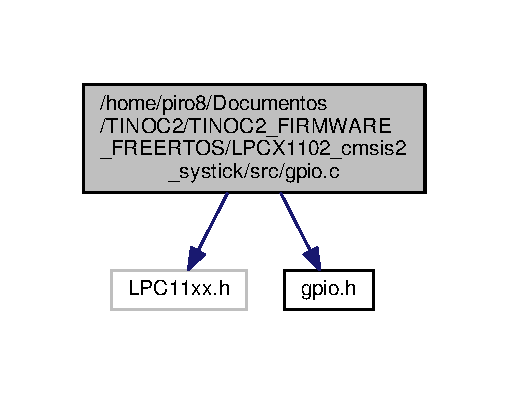
\includegraphics[width=226pt]{gpio_8c__incl}
\end{center}
\end{figure}
\subsection*{Functions}
\begin{DoxyCompactItemize}
\item 
void \hyperlink{gpio_8c_a82d16a95aba432b8eb2464734a1c79a6}{G\+P\+I\+O\+Init} (void)
\item 
void \hyperlink{gpio_8c_a376642dd36001cc5eb409f9c83152e60}{G\+P\+I\+O\+Set\+Dir} (uint32\+\_\+t port\+Num, uint32\+\_\+t bit\+Posi, uint32\+\_\+t dir)
\item 
void \hyperlink{gpio_8c_a6e2440fb6429a69f1338b51a4cab2921}{G\+P\+I\+O\+Set\+Value} (uint32\+\_\+t port\+Num, uint32\+\_\+t bit\+Posi, uint32\+\_\+t bit\+Val)
\item 
void \hyperlink{gpio_8c_a3a32c210c15bc18c66b21d1dc954cc0f}{G\+P\+I\+O\+Set\+Interrupt} (uint32\+\_\+t port\+Num, uint32\+\_\+t bit\+Posi, uint32\+\_\+t sense, uint32\+\_\+t single, uint32\+\_\+t event)
\item 
void \hyperlink{gpio_8c_ac500e8eefbe2b7216d438c08b7f9db0f}{G\+P\+I\+O\+Int\+Enable} (uint32\+\_\+t port\+Num, uint32\+\_\+t bit\+Posi)
\item 
void \hyperlink{gpio_8c_a4f7f9fbe0f93649e73771327cfcb17e9}{G\+P\+I\+O\+Int\+Disable} (uint32\+\_\+t port\+Num, uint32\+\_\+t bit\+Posi)
\item 
uint32\+\_\+t \hyperlink{gpio_8c_a384e59b5b114d369e639206cc1e87e2f}{G\+P\+I\+O\+Int\+Status} (uint32\+\_\+t port\+Num, uint32\+\_\+t bit\+Posi)
\item 
void \hyperlink{gpio_8c_a2e99ceb76757e9ecb2c9a4562839d90e}{G\+P\+I\+O\+Int\+Clear} (uint32\+\_\+t port\+Num, uint32\+\_\+t bit\+Posi)
\end{DoxyCompactItemize}


\subsection{Detailed Description}
G\+P\+IO C file for N\+XP L\+P\+C11xx Family Microprocessors. 

~\newline
 History \begin{DoxyItemize}
\item 2009.\+12.\+09 ver 1.\+01 \hyperlink{gpio_8c_a6e2440fb6429a69f1338b51a4cab2921}{G\+P\+I\+O\+Set\+Value()} updated \item 2008.\+07.\+20 ver 1.\+00 Preliminary version, first Release\end{DoxyItemize}
\begin{DoxyAuthor}{Author}
Copyright(\+C) 2008, N\+XP Semiconductor. All rights reserved. 

Roux, Federico G. (\href{mailto:froux@citedef.gob.ar}{\tt froux@citedef.\+gob.\+ar}). C\+I\+T\+E\+D\+E\+F2014 
\end{DoxyAuthor}


\subsection{Function Documentation}
\index{gpio.\+c@{gpio.\+c}!G\+P\+I\+O\+Init@{G\+P\+I\+O\+Init}}
\index{G\+P\+I\+O\+Init@{G\+P\+I\+O\+Init}!gpio.\+c@{gpio.\+c}}
\subsubsection[{\texorpdfstring{G\+P\+I\+O\+Init(void)}{GPIOInit(void)}}]{\setlength{\rightskip}{0pt plus 5cm}void G\+P\+I\+O\+Init (
\begin{DoxyParamCaption}
\item[{void}]{}
\end{DoxyParamCaption}
)}\hypertarget{gpio_8c_a82d16a95aba432b8eb2464734a1c79a6}{}\label{gpio_8c_a82d16a95aba432b8eb2464734a1c79a6}
Function name\+: G\+P\+I\+O\+Init

Descriptions\+: Initialize G\+P\+IO, install the G\+P\+IO interrupt handler

parameters\+: None Returned value\+: true or false, return false if the V\+IC table is full and G\+P\+IO interrupt handler can be installed. 

Definition at line 142 of file gpio.\+c.

\index{gpio.\+c@{gpio.\+c}!G\+P\+I\+O\+Int\+Clear@{G\+P\+I\+O\+Int\+Clear}}
\index{G\+P\+I\+O\+Int\+Clear@{G\+P\+I\+O\+Int\+Clear}!gpio.\+c@{gpio.\+c}}
\subsubsection[{\texorpdfstring{G\+P\+I\+O\+Int\+Clear(uint32\+\_\+t port\+Num, uint32\+\_\+t bit\+Posi)}{GPIOIntClear(uint32_t portNum, uint32_t bitPosi)}}]{\setlength{\rightskip}{0pt plus 5cm}void G\+P\+I\+O\+Int\+Clear (
\begin{DoxyParamCaption}
\item[{uint32\+\_\+t}]{port\+Num, }
\item[{uint32\+\_\+t}]{bit\+Posi}
\end{DoxyParamCaption}
)}\hypertarget{gpio_8c_a2e99ceb76757e9ecb2c9a4562839d90e}{}\label{gpio_8c_a2e99ceb76757e9ecb2c9a4562839d90e}


Definition at line 454 of file gpio.\+c.

\index{gpio.\+c@{gpio.\+c}!G\+P\+I\+O\+Int\+Disable@{G\+P\+I\+O\+Int\+Disable}}
\index{G\+P\+I\+O\+Int\+Disable@{G\+P\+I\+O\+Int\+Disable}!gpio.\+c@{gpio.\+c}}
\subsubsection[{\texorpdfstring{G\+P\+I\+O\+Int\+Disable(uint32\+\_\+t port\+Num, uint32\+\_\+t bit\+Posi)}{GPIOIntDisable(uint32_t portNum, uint32_t bitPosi)}}]{\setlength{\rightskip}{0pt plus 5cm}void G\+P\+I\+O\+Int\+Disable (
\begin{DoxyParamCaption}
\item[{uint32\+\_\+t}]{port\+Num, }
\item[{uint32\+\_\+t}]{bit\+Posi}
\end{DoxyParamCaption}
)}\hypertarget{gpio_8c_a4f7f9fbe0f93649e73771327cfcb17e9}{}\label{gpio_8c_a4f7f9fbe0f93649e73771327cfcb17e9}


Definition at line 386 of file gpio.\+c.

\index{gpio.\+c@{gpio.\+c}!G\+P\+I\+O\+Int\+Enable@{G\+P\+I\+O\+Int\+Enable}}
\index{G\+P\+I\+O\+Int\+Enable@{G\+P\+I\+O\+Int\+Enable}!gpio.\+c@{gpio.\+c}}
\subsubsection[{\texorpdfstring{G\+P\+I\+O\+Int\+Enable(uint32\+\_\+t port\+Num, uint32\+\_\+t bit\+Posi)}{GPIOIntEnable(uint32_t portNum, uint32_t bitPosi)}}]{\setlength{\rightskip}{0pt plus 5cm}void G\+P\+I\+O\+Int\+Enable (
\begin{DoxyParamCaption}
\item[{uint32\+\_\+t}]{port\+Num, }
\item[{uint32\+\_\+t}]{bit\+Posi}
\end{DoxyParamCaption}
)}\hypertarget{gpio_8c_ac500e8eefbe2b7216d438c08b7f9db0f}{}\label{gpio_8c_ac500e8eefbe2b7216d438c08b7f9db0f}


Definition at line 355 of file gpio.\+c.

\index{gpio.\+c@{gpio.\+c}!G\+P\+I\+O\+Int\+Status@{G\+P\+I\+O\+Int\+Status}}
\index{G\+P\+I\+O\+Int\+Status@{G\+P\+I\+O\+Int\+Status}!gpio.\+c@{gpio.\+c}}
\subsubsection[{\texorpdfstring{G\+P\+I\+O\+Int\+Status(uint32\+\_\+t port\+Num, uint32\+\_\+t bit\+Posi)}{GPIOIntStatus(uint32_t portNum, uint32_t bitPosi)}}]{\setlength{\rightskip}{0pt plus 5cm}uint32\+\_\+t G\+P\+I\+O\+Int\+Status (
\begin{DoxyParamCaption}
\item[{uint32\+\_\+t}]{port\+Num, }
\item[{uint32\+\_\+t}]{bit\+Posi}
\end{DoxyParamCaption}
)}\hypertarget{gpio_8c_a384e59b5b114d369e639206cc1e87e2f}{}\label{gpio_8c_a384e59b5b114d369e639206cc1e87e2f}


Definition at line 417 of file gpio.\+c.

\index{gpio.\+c@{gpio.\+c}!G\+P\+I\+O\+Set\+Dir@{G\+P\+I\+O\+Set\+Dir}}
\index{G\+P\+I\+O\+Set\+Dir@{G\+P\+I\+O\+Set\+Dir}!gpio.\+c@{gpio.\+c}}
\subsubsection[{\texorpdfstring{G\+P\+I\+O\+Set\+Dir(uint32\+\_\+t port\+Num, uint32\+\_\+t bit\+Posi, uint32\+\_\+t dir)}{GPIOSetDir(uint32_t portNum, uint32_t bitPosi, uint32_t dir)}}]{\setlength{\rightskip}{0pt plus 5cm}void G\+P\+I\+O\+Set\+Dir (
\begin{DoxyParamCaption}
\item[{uint32\+\_\+t}]{port\+Num, }
\item[{uint32\+\_\+t}]{bit\+Posi, }
\item[{uint32\+\_\+t}]{dir}
\end{DoxyParamCaption}
)}\hypertarget{gpio_8c_a376642dd36001cc5eb409f9c83152e60}{}\label{gpio_8c_a376642dd36001cc5eb409f9c83152e60}


Definition at line 169 of file gpio.\+c.

\index{gpio.\+c@{gpio.\+c}!G\+P\+I\+O\+Set\+Interrupt@{G\+P\+I\+O\+Set\+Interrupt}}
\index{G\+P\+I\+O\+Set\+Interrupt@{G\+P\+I\+O\+Set\+Interrupt}!gpio.\+c@{gpio.\+c}}
\subsubsection[{\texorpdfstring{G\+P\+I\+O\+Set\+Interrupt(uint32\+\_\+t port\+Num, uint32\+\_\+t bit\+Posi, uint32\+\_\+t sense, uint32\+\_\+t single, uint32\+\_\+t event)}{GPIOSetInterrupt(uint32_t portNum, uint32_t bitPosi, uint32_t sense, uint32_t single, uint32_t event)}}]{\setlength{\rightskip}{0pt plus 5cm}void G\+P\+I\+O\+Set\+Interrupt (
\begin{DoxyParamCaption}
\item[{uint32\+\_\+t}]{port\+Num, }
\item[{uint32\+\_\+t}]{bit\+Posi, }
\item[{uint32\+\_\+t}]{sense, }
\item[{uint32\+\_\+t}]{single, }
\item[{uint32\+\_\+t}]{event}
\end{DoxyParamCaption}
)}\hypertarget{gpio_8c_a3a32c210c15bc18c66b21d1dc954cc0f}{}\label{gpio_8c_a3a32c210c15bc18c66b21d1dc954cc0f}


Definition at line 267 of file gpio.\+c.

\index{gpio.\+c@{gpio.\+c}!G\+P\+I\+O\+Set\+Value@{G\+P\+I\+O\+Set\+Value}}
\index{G\+P\+I\+O\+Set\+Value@{G\+P\+I\+O\+Set\+Value}!gpio.\+c@{gpio.\+c}}
\subsubsection[{\texorpdfstring{G\+P\+I\+O\+Set\+Value(uint32\+\_\+t port\+Num, uint32\+\_\+t bit\+Posi, uint32\+\_\+t bit\+Val)}{GPIOSetValue(uint32_t portNum, uint32_t bitPosi, uint32_t bitVal)}}]{\setlength{\rightskip}{0pt plus 5cm}void G\+P\+I\+O\+Set\+Value (
\begin{DoxyParamCaption}
\item[{uint32\+\_\+t}]{port\+Num, }
\item[{uint32\+\_\+t}]{bit\+Posi, }
\item[{uint32\+\_\+t}]{bit\+Val}
\end{DoxyParamCaption}
)}\hypertarget{gpio_8c_a6e2440fb6429a69f1338b51a4cab2921}{}\label{gpio_8c_a6e2440fb6429a69f1338b51a4cab2921}


Definition at line 218 of file gpio.\+c.


\hypertarget{gpio_8h}{}\section{/home/telemetria/git/workspaces/tinoc2\+\_\+firmware\+\_\+freertos/\+R\+T\+O\+S\+Demo/\+Source/gpio/gpio.h File Reference}
\label{gpio_8h}\index{/home/telemetria/git/workspaces/tinoc2\+\_\+firmware\+\_\+freertos/\+R\+T\+O\+S\+Demo/\+Source/gpio/gpio.\+h@{/home/telemetria/git/workspaces/tinoc2\+\_\+firmware\+\_\+freertos/\+R\+T\+O\+S\+Demo/\+Source/gpio/gpio.\+h}}
This graph shows which files directly or indirectly include this file\+:
\nopagebreak
\begin{figure}[H]
\begin{center}
\leavevmode
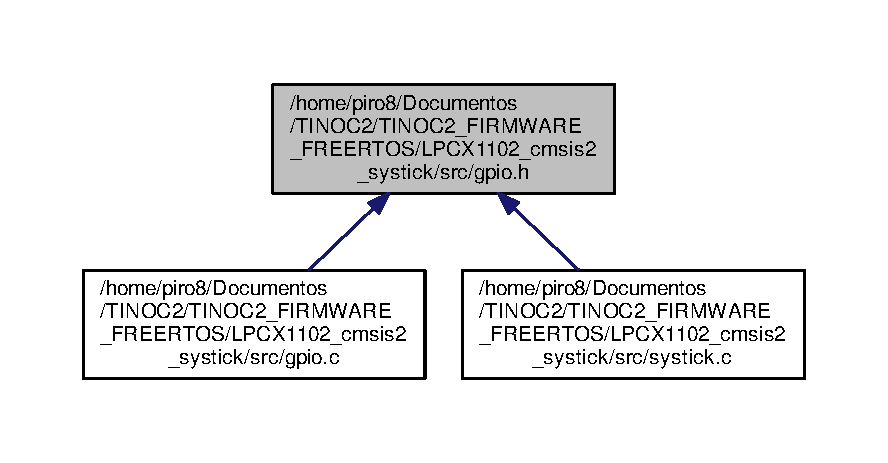
\includegraphics[width=350pt]{gpio_8h__dep__incl}
\end{center}
\end{figure}
\subsection*{Macros}
\begin{DoxyCompactItemize}
\item 
\#define \hyperlink{gpio_8h_af41b34488a518db05b413d3a370f871f}{P\+O\+R\+T0}~0
\item 
\#define \hyperlink{gpio_8h_a83b698b796fa8d1625536439f28ea575}{P\+O\+R\+T1}~1
\item 
\#define \hyperlink{gpio_8h_acb270e4aec8a0ab123e6c24a5810150b}{P\+O\+R\+T2}~2
\item 
\#define \hyperlink{gpio_8h_ad906b7f6a811f1f02b5eb04cbe1bc89b}{P\+O\+R\+T3}~3
\item 
\#define \hyperlink{gpio_8h_a718485b7da5da3428aeaa13999868328}{G\+P\+I\+O\+\_\+\+E\+N\+T\+R\+A\+DA}~0
\item 
\#define \hyperlink{gpio_8h_af0b02248c9da7e0d37a5f215125d2c40}{G\+P\+I\+O\+\_\+\+S\+A\+L\+I\+DA}~1
\item 
\#define \hyperlink{gpio_8h_a80dde28b73c4b23792432750d7315cf6}{G\+P\+I\+O\+\_\+\+I\+S\+\_\+\+E\+D\+GE}~0
\item 
\#define \hyperlink{gpio_8h_a77cfb813d4266e7e76399b56a4f04af5}{G\+P\+I\+O\+\_\+\+I\+S\+\_\+\+L\+E\+V\+EL}~1
\item 
\#define \hyperlink{gpio_8h_a514332d080e218dcb68c0158eaff3c9a}{G\+P\+I\+O\+\_\+\+I\+E\+V\+\_\+\+N\+I\+V\+E\+L\+\_\+\+B\+A\+JO}~0
\item 
\#define \hyperlink{gpio_8h_a2c9b1519dbbb588b80b9aaaa844e2068}{G\+P\+I\+O\+\_\+\+I\+E\+V\+\_\+\+F\+L\+A\+N\+C\+O\+\_\+\+B\+A\+J\+A\+DA}~0
\item 
\#define \hyperlink{gpio_8h_ac9746ce49e0e7b9e1bd50d2190e7f80d}{G\+P\+I\+O\+\_\+\+I\+E\+V\+\_\+\+N\+I\+V\+E\+L\+\_\+\+A\+L\+TO}~1
\item 
\#define \hyperlink{gpio_8h_a66390c69175e06b4b099f6670a18ba86}{G\+P\+I\+O\+\_\+\+I\+E\+V\+\_\+\+F\+L\+A\+N\+C\+O\+\_\+\+S\+U\+B\+I\+DA}~1
\item 
\#define \hyperlink{gpio_8h_a25827f27403b49901b49759bdf85e9bc}{G\+P\+I\+O\+\_\+\+I\+B\+E\+\_\+\+C\+O\+N\+T\+R\+O\+L\+\_\+\+I\+EV}~0
\item 
\#define \hyperlink{gpio_8h_a2b8eb0b9e55f183eb1afaa80a5bf237e}{G\+P\+I\+O\+\_\+\+I\+B\+E\+\_\+\+C\+O\+N\+T\+R\+O\+L\+\_\+\+B\+O\+TH}~1
\end{DoxyCompactItemize}
\subsection*{Functions}
\begin{DoxyCompactItemize}
\item 
void \hyperlink{gpio_8h_abba8cf772801f0270a6fc168849161b8}{G\+P\+I\+O\+\_\+\+I\+R\+Q\+Handler} (void)
\item 
void \hyperlink{gpio_8h_a82d16a95aba432b8eb2464734a1c79a6}{G\+P\+I\+O\+Init} (void)
\item 
void \hyperlink{gpio_8h_a376642dd36001cc5eb409f9c83152e60}{G\+P\+I\+O\+Set\+Dir} (uint32\+\_\+t port\+Num, uint32\+\_\+t bit\+Posi, uint32\+\_\+t dir)
\item 
void \hyperlink{gpio_8h_a6e2440fb6429a69f1338b51a4cab2921}{G\+P\+I\+O\+Set\+Value} (uint32\+\_\+t port\+Num, uint32\+\_\+t bit\+Posi, uint32\+\_\+t bit\+Val)
\item 
void \hyperlink{gpio_8h_a3a32c210c15bc18c66b21d1dc954cc0f}{G\+P\+I\+O\+Set\+Interrupt} (uint32\+\_\+t port\+Num, uint32\+\_\+t bit\+Posi, uint32\+\_\+t sense, uint32\+\_\+t single, uint32\+\_\+t event)
\item 
void \hyperlink{gpio_8h_ac500e8eefbe2b7216d438c08b7f9db0f}{G\+P\+I\+O\+Int\+Enable} (uint32\+\_\+t port\+Num, uint32\+\_\+t bit\+Posi)
\item 
void \hyperlink{gpio_8h_a4f7f9fbe0f93649e73771327cfcb17e9}{G\+P\+I\+O\+Int\+Disable} (uint32\+\_\+t port\+Num, uint32\+\_\+t bit\+Posi)
\item 
uint32\+\_\+t \hyperlink{gpio_8h_a384e59b5b114d369e639206cc1e87e2f}{G\+P\+I\+O\+Int\+Status} (uint32\+\_\+t port\+Num, uint32\+\_\+t bit\+Posi)
\item 
void \hyperlink{gpio_8h_a2e99ceb76757e9ecb2c9a4562839d90e}{G\+P\+I\+O\+Int\+Clear} (uint32\+\_\+t port\+Num, uint32\+\_\+t bit\+Posi)
\end{DoxyCompactItemize}


\subsection{Macro Definition Documentation}
\index{gpio.\+h@{gpio.\+h}!G\+P\+I\+O\+\_\+\+E\+N\+T\+R\+A\+DA@{G\+P\+I\+O\+\_\+\+E\+N\+T\+R\+A\+DA}}
\index{G\+P\+I\+O\+\_\+\+E\+N\+T\+R\+A\+DA@{G\+P\+I\+O\+\_\+\+E\+N\+T\+R\+A\+DA}!gpio.\+h@{gpio.\+h}}
\subsubsection[{\texorpdfstring{G\+P\+I\+O\+\_\+\+E\+N\+T\+R\+A\+DA}{GPIO_ENTRADA}}]{\setlength{\rightskip}{0pt plus 5cm}\#define G\+P\+I\+O\+\_\+\+E\+N\+T\+R\+A\+DA~0}\hypertarget{gpio_8h_a718485b7da5da3428aeaa13999868328}{}\label{gpio_8h_a718485b7da5da3428aeaa13999868328}


Definition at line 24 of file gpio.\+h.

\index{gpio.\+h@{gpio.\+h}!G\+P\+I\+O\+\_\+\+I\+B\+E\+\_\+\+C\+O\+N\+T\+R\+O\+L\+\_\+\+B\+O\+TH@{G\+P\+I\+O\+\_\+\+I\+B\+E\+\_\+\+C\+O\+N\+T\+R\+O\+L\+\_\+\+B\+O\+TH}}
\index{G\+P\+I\+O\+\_\+\+I\+B\+E\+\_\+\+C\+O\+N\+T\+R\+O\+L\+\_\+\+B\+O\+TH@{G\+P\+I\+O\+\_\+\+I\+B\+E\+\_\+\+C\+O\+N\+T\+R\+O\+L\+\_\+\+B\+O\+TH}!gpio.\+h@{gpio.\+h}}
\subsubsection[{\texorpdfstring{G\+P\+I\+O\+\_\+\+I\+B\+E\+\_\+\+C\+O\+N\+T\+R\+O\+L\+\_\+\+B\+O\+TH}{GPIO_IBE_CONTROL_BOTH}}]{\setlength{\rightskip}{0pt plus 5cm}\#define G\+P\+I\+O\+\_\+\+I\+B\+E\+\_\+\+C\+O\+N\+T\+R\+O\+L\+\_\+\+B\+O\+TH~1}\hypertarget{gpio_8h_a2b8eb0b9e55f183eb1afaa80a5bf237e}{}\label{gpio_8h_a2b8eb0b9e55f183eb1afaa80a5bf237e}


Definition at line 36 of file gpio.\+h.

\index{gpio.\+h@{gpio.\+h}!G\+P\+I\+O\+\_\+\+I\+B\+E\+\_\+\+C\+O\+N\+T\+R\+O\+L\+\_\+\+I\+EV@{G\+P\+I\+O\+\_\+\+I\+B\+E\+\_\+\+C\+O\+N\+T\+R\+O\+L\+\_\+\+I\+EV}}
\index{G\+P\+I\+O\+\_\+\+I\+B\+E\+\_\+\+C\+O\+N\+T\+R\+O\+L\+\_\+\+I\+EV@{G\+P\+I\+O\+\_\+\+I\+B\+E\+\_\+\+C\+O\+N\+T\+R\+O\+L\+\_\+\+I\+EV}!gpio.\+h@{gpio.\+h}}
\subsubsection[{\texorpdfstring{G\+P\+I\+O\+\_\+\+I\+B\+E\+\_\+\+C\+O\+N\+T\+R\+O\+L\+\_\+\+I\+EV}{GPIO_IBE_CONTROL_IEV}}]{\setlength{\rightskip}{0pt plus 5cm}\#define G\+P\+I\+O\+\_\+\+I\+B\+E\+\_\+\+C\+O\+N\+T\+R\+O\+L\+\_\+\+I\+EV~0}\hypertarget{gpio_8h_a25827f27403b49901b49759bdf85e9bc}{}\label{gpio_8h_a25827f27403b49901b49759bdf85e9bc}


Definition at line 35 of file gpio.\+h.

\index{gpio.\+h@{gpio.\+h}!G\+P\+I\+O\+\_\+\+I\+E\+V\+\_\+\+F\+L\+A\+N\+C\+O\+\_\+\+B\+A\+J\+A\+DA@{G\+P\+I\+O\+\_\+\+I\+E\+V\+\_\+\+F\+L\+A\+N\+C\+O\+\_\+\+B\+A\+J\+A\+DA}}
\index{G\+P\+I\+O\+\_\+\+I\+E\+V\+\_\+\+F\+L\+A\+N\+C\+O\+\_\+\+B\+A\+J\+A\+DA@{G\+P\+I\+O\+\_\+\+I\+E\+V\+\_\+\+F\+L\+A\+N\+C\+O\+\_\+\+B\+A\+J\+A\+DA}!gpio.\+h@{gpio.\+h}}
\subsubsection[{\texorpdfstring{G\+P\+I\+O\+\_\+\+I\+E\+V\+\_\+\+F\+L\+A\+N\+C\+O\+\_\+\+B\+A\+J\+A\+DA}{GPIO_IEV_FLANCO_BAJADA}}]{\setlength{\rightskip}{0pt plus 5cm}\#define G\+P\+I\+O\+\_\+\+I\+E\+V\+\_\+\+F\+L\+A\+N\+C\+O\+\_\+\+B\+A\+J\+A\+DA~0}\hypertarget{gpio_8h_a2c9b1519dbbb588b80b9aaaa844e2068}{}\label{gpio_8h_a2c9b1519dbbb588b80b9aaaa844e2068}


Definition at line 31 of file gpio.\+h.

\index{gpio.\+h@{gpio.\+h}!G\+P\+I\+O\+\_\+\+I\+E\+V\+\_\+\+F\+L\+A\+N\+C\+O\+\_\+\+S\+U\+B\+I\+DA@{G\+P\+I\+O\+\_\+\+I\+E\+V\+\_\+\+F\+L\+A\+N\+C\+O\+\_\+\+S\+U\+B\+I\+DA}}
\index{G\+P\+I\+O\+\_\+\+I\+E\+V\+\_\+\+F\+L\+A\+N\+C\+O\+\_\+\+S\+U\+B\+I\+DA@{G\+P\+I\+O\+\_\+\+I\+E\+V\+\_\+\+F\+L\+A\+N\+C\+O\+\_\+\+S\+U\+B\+I\+DA}!gpio.\+h@{gpio.\+h}}
\subsubsection[{\texorpdfstring{G\+P\+I\+O\+\_\+\+I\+E\+V\+\_\+\+F\+L\+A\+N\+C\+O\+\_\+\+S\+U\+B\+I\+DA}{GPIO_IEV_FLANCO_SUBIDA}}]{\setlength{\rightskip}{0pt plus 5cm}\#define G\+P\+I\+O\+\_\+\+I\+E\+V\+\_\+\+F\+L\+A\+N\+C\+O\+\_\+\+S\+U\+B\+I\+DA~1}\hypertarget{gpio_8h_a66390c69175e06b4b099f6670a18ba86}{}\label{gpio_8h_a66390c69175e06b4b099f6670a18ba86}


Definition at line 33 of file gpio.\+h.

\index{gpio.\+h@{gpio.\+h}!G\+P\+I\+O\+\_\+\+I\+E\+V\+\_\+\+N\+I\+V\+E\+L\+\_\+\+A\+L\+TO@{G\+P\+I\+O\+\_\+\+I\+E\+V\+\_\+\+N\+I\+V\+E\+L\+\_\+\+A\+L\+TO}}
\index{G\+P\+I\+O\+\_\+\+I\+E\+V\+\_\+\+N\+I\+V\+E\+L\+\_\+\+A\+L\+TO@{G\+P\+I\+O\+\_\+\+I\+E\+V\+\_\+\+N\+I\+V\+E\+L\+\_\+\+A\+L\+TO}!gpio.\+h@{gpio.\+h}}
\subsubsection[{\texorpdfstring{G\+P\+I\+O\+\_\+\+I\+E\+V\+\_\+\+N\+I\+V\+E\+L\+\_\+\+A\+L\+TO}{GPIO_IEV_NIVEL_ALTO}}]{\setlength{\rightskip}{0pt plus 5cm}\#define G\+P\+I\+O\+\_\+\+I\+E\+V\+\_\+\+N\+I\+V\+E\+L\+\_\+\+A\+L\+TO~1}\hypertarget{gpio_8h_ac9746ce49e0e7b9e1bd50d2190e7f80d}{}\label{gpio_8h_ac9746ce49e0e7b9e1bd50d2190e7f80d}


Definition at line 32 of file gpio.\+h.

\index{gpio.\+h@{gpio.\+h}!G\+P\+I\+O\+\_\+\+I\+E\+V\+\_\+\+N\+I\+V\+E\+L\+\_\+\+B\+A\+JO@{G\+P\+I\+O\+\_\+\+I\+E\+V\+\_\+\+N\+I\+V\+E\+L\+\_\+\+B\+A\+JO}}
\index{G\+P\+I\+O\+\_\+\+I\+E\+V\+\_\+\+N\+I\+V\+E\+L\+\_\+\+B\+A\+JO@{G\+P\+I\+O\+\_\+\+I\+E\+V\+\_\+\+N\+I\+V\+E\+L\+\_\+\+B\+A\+JO}!gpio.\+h@{gpio.\+h}}
\subsubsection[{\texorpdfstring{G\+P\+I\+O\+\_\+\+I\+E\+V\+\_\+\+N\+I\+V\+E\+L\+\_\+\+B\+A\+JO}{GPIO_IEV_NIVEL_BAJO}}]{\setlength{\rightskip}{0pt plus 5cm}\#define G\+P\+I\+O\+\_\+\+I\+E\+V\+\_\+\+N\+I\+V\+E\+L\+\_\+\+B\+A\+JO~0}\hypertarget{gpio_8h_a514332d080e218dcb68c0158eaff3c9a}{}\label{gpio_8h_a514332d080e218dcb68c0158eaff3c9a}


Definition at line 30 of file gpio.\+h.

\index{gpio.\+h@{gpio.\+h}!G\+P\+I\+O\+\_\+\+I\+S\+\_\+\+E\+D\+GE@{G\+P\+I\+O\+\_\+\+I\+S\+\_\+\+E\+D\+GE}}
\index{G\+P\+I\+O\+\_\+\+I\+S\+\_\+\+E\+D\+GE@{G\+P\+I\+O\+\_\+\+I\+S\+\_\+\+E\+D\+GE}!gpio.\+h@{gpio.\+h}}
\subsubsection[{\texorpdfstring{G\+P\+I\+O\+\_\+\+I\+S\+\_\+\+E\+D\+GE}{GPIO_IS_EDGE}}]{\setlength{\rightskip}{0pt plus 5cm}\#define G\+P\+I\+O\+\_\+\+I\+S\+\_\+\+E\+D\+GE~0}\hypertarget{gpio_8h_a80dde28b73c4b23792432750d7315cf6}{}\label{gpio_8h_a80dde28b73c4b23792432750d7315cf6}


Definition at line 27 of file gpio.\+h.

\index{gpio.\+h@{gpio.\+h}!G\+P\+I\+O\+\_\+\+I\+S\+\_\+\+L\+E\+V\+EL@{G\+P\+I\+O\+\_\+\+I\+S\+\_\+\+L\+E\+V\+EL}}
\index{G\+P\+I\+O\+\_\+\+I\+S\+\_\+\+L\+E\+V\+EL@{G\+P\+I\+O\+\_\+\+I\+S\+\_\+\+L\+E\+V\+EL}!gpio.\+h@{gpio.\+h}}
\subsubsection[{\texorpdfstring{G\+P\+I\+O\+\_\+\+I\+S\+\_\+\+L\+E\+V\+EL}{GPIO_IS_LEVEL}}]{\setlength{\rightskip}{0pt plus 5cm}\#define G\+P\+I\+O\+\_\+\+I\+S\+\_\+\+L\+E\+V\+EL~1}\hypertarget{gpio_8h_a77cfb813d4266e7e76399b56a4f04af5}{}\label{gpio_8h_a77cfb813d4266e7e76399b56a4f04af5}


Definition at line 28 of file gpio.\+h.

\index{gpio.\+h@{gpio.\+h}!G\+P\+I\+O\+\_\+\+S\+A\+L\+I\+DA@{G\+P\+I\+O\+\_\+\+S\+A\+L\+I\+DA}}
\index{G\+P\+I\+O\+\_\+\+S\+A\+L\+I\+DA@{G\+P\+I\+O\+\_\+\+S\+A\+L\+I\+DA}!gpio.\+h@{gpio.\+h}}
\subsubsection[{\texorpdfstring{G\+P\+I\+O\+\_\+\+S\+A\+L\+I\+DA}{GPIO_SALIDA}}]{\setlength{\rightskip}{0pt plus 5cm}\#define G\+P\+I\+O\+\_\+\+S\+A\+L\+I\+DA~1}\hypertarget{gpio_8h_af0b02248c9da7e0d37a5f215125d2c40}{}\label{gpio_8h_af0b02248c9da7e0d37a5f215125d2c40}


Definition at line 25 of file gpio.\+h.

\index{gpio.\+h@{gpio.\+h}!P\+O\+R\+T0@{P\+O\+R\+T0}}
\index{P\+O\+R\+T0@{P\+O\+R\+T0}!gpio.\+h@{gpio.\+h}}
\subsubsection[{\texorpdfstring{P\+O\+R\+T0}{PORT0}}]{\setlength{\rightskip}{0pt plus 5cm}\#define P\+O\+R\+T0~0}\hypertarget{gpio_8h_af41b34488a518db05b413d3a370f871f}{}\label{gpio_8h_af41b34488a518db05b413d3a370f871f}


Definition at line 19 of file gpio.\+h.

\index{gpio.\+h@{gpio.\+h}!P\+O\+R\+T1@{P\+O\+R\+T1}}
\index{P\+O\+R\+T1@{P\+O\+R\+T1}!gpio.\+h@{gpio.\+h}}
\subsubsection[{\texorpdfstring{P\+O\+R\+T1}{PORT1}}]{\setlength{\rightskip}{0pt plus 5cm}\#define P\+O\+R\+T1~1}\hypertarget{gpio_8h_a83b698b796fa8d1625536439f28ea575}{}\label{gpio_8h_a83b698b796fa8d1625536439f28ea575}


Definition at line 20 of file gpio.\+h.

\index{gpio.\+h@{gpio.\+h}!P\+O\+R\+T2@{P\+O\+R\+T2}}
\index{P\+O\+R\+T2@{P\+O\+R\+T2}!gpio.\+h@{gpio.\+h}}
\subsubsection[{\texorpdfstring{P\+O\+R\+T2}{PORT2}}]{\setlength{\rightskip}{0pt plus 5cm}\#define P\+O\+R\+T2~2}\hypertarget{gpio_8h_acb270e4aec8a0ab123e6c24a5810150b}{}\label{gpio_8h_acb270e4aec8a0ab123e6c24a5810150b}


Definition at line 21 of file gpio.\+h.

\index{gpio.\+h@{gpio.\+h}!P\+O\+R\+T3@{P\+O\+R\+T3}}
\index{P\+O\+R\+T3@{P\+O\+R\+T3}!gpio.\+h@{gpio.\+h}}
\subsubsection[{\texorpdfstring{P\+O\+R\+T3}{PORT3}}]{\setlength{\rightskip}{0pt plus 5cm}\#define P\+O\+R\+T3~3}\hypertarget{gpio_8h_ad906b7f6a811f1f02b5eb04cbe1bc89b}{}\label{gpio_8h_ad906b7f6a811f1f02b5eb04cbe1bc89b}


Definition at line 22 of file gpio.\+h.



\subsection{Function Documentation}
\index{gpio.\+h@{gpio.\+h}!G\+P\+I\+O\+\_\+\+I\+R\+Q\+Handler@{G\+P\+I\+O\+\_\+\+I\+R\+Q\+Handler}}
\index{G\+P\+I\+O\+\_\+\+I\+R\+Q\+Handler@{G\+P\+I\+O\+\_\+\+I\+R\+Q\+Handler}!gpio.\+h@{gpio.\+h}}
\subsubsection[{\texorpdfstring{G\+P\+I\+O\+\_\+\+I\+R\+Q\+Handler(void)}{GPIO_IRQHandler(void)}}]{\setlength{\rightskip}{0pt plus 5cm}void G\+P\+I\+O\+\_\+\+I\+R\+Q\+Handler (
\begin{DoxyParamCaption}
\item[{void}]{}
\end{DoxyParamCaption}
)}\hypertarget{gpio_8h_abba8cf772801f0270a6fc168849161b8}{}\label{gpio_8h_abba8cf772801f0270a6fc168849161b8}
\index{gpio.\+h@{gpio.\+h}!G\+P\+I\+O\+Init@{G\+P\+I\+O\+Init}}
\index{G\+P\+I\+O\+Init@{G\+P\+I\+O\+Init}!gpio.\+h@{gpio.\+h}}
\subsubsection[{\texorpdfstring{G\+P\+I\+O\+Init(void)}{GPIOInit(void)}}]{\setlength{\rightskip}{0pt plus 5cm}void G\+P\+I\+O\+Init (
\begin{DoxyParamCaption}
\item[{void}]{}
\end{DoxyParamCaption}
)}\hypertarget{gpio_8h_a82d16a95aba432b8eb2464734a1c79a6}{}\label{gpio_8h_a82d16a95aba432b8eb2464734a1c79a6}
Function name\+: G\+P\+I\+O\+Init

Descriptions\+: Initialize G\+P\+IO, install the G\+P\+IO interrupt handler

parameters\+: None Returned value\+: true or false, return false if the V\+IC table is full and G\+P\+IO interrupt handler can be installed. 

Definition at line 142 of file gpio.\+c.

\index{gpio.\+h@{gpio.\+h}!G\+P\+I\+O\+Int\+Clear@{G\+P\+I\+O\+Int\+Clear}}
\index{G\+P\+I\+O\+Int\+Clear@{G\+P\+I\+O\+Int\+Clear}!gpio.\+h@{gpio.\+h}}
\subsubsection[{\texorpdfstring{G\+P\+I\+O\+Int\+Clear(uint32\+\_\+t port\+Num, uint32\+\_\+t bit\+Posi)}{GPIOIntClear(uint32_t portNum, uint32_t bitPosi)}}]{\setlength{\rightskip}{0pt plus 5cm}void G\+P\+I\+O\+Int\+Clear (
\begin{DoxyParamCaption}
\item[{uint32\+\_\+t}]{port\+Num, }
\item[{uint32\+\_\+t}]{bit\+Posi}
\end{DoxyParamCaption}
)}\hypertarget{gpio_8h_a2e99ceb76757e9ecb2c9a4562839d90e}{}\label{gpio_8h_a2e99ceb76757e9ecb2c9a4562839d90e}


Definition at line 454 of file gpio.\+c.

\index{gpio.\+h@{gpio.\+h}!G\+P\+I\+O\+Int\+Disable@{G\+P\+I\+O\+Int\+Disable}}
\index{G\+P\+I\+O\+Int\+Disable@{G\+P\+I\+O\+Int\+Disable}!gpio.\+h@{gpio.\+h}}
\subsubsection[{\texorpdfstring{G\+P\+I\+O\+Int\+Disable(uint32\+\_\+t port\+Num, uint32\+\_\+t bit\+Posi)}{GPIOIntDisable(uint32_t portNum, uint32_t bitPosi)}}]{\setlength{\rightskip}{0pt plus 5cm}void G\+P\+I\+O\+Int\+Disable (
\begin{DoxyParamCaption}
\item[{uint32\+\_\+t}]{port\+Num, }
\item[{uint32\+\_\+t}]{bit\+Posi}
\end{DoxyParamCaption}
)}\hypertarget{gpio_8h_a4f7f9fbe0f93649e73771327cfcb17e9}{}\label{gpio_8h_a4f7f9fbe0f93649e73771327cfcb17e9}


Definition at line 386 of file gpio.\+c.

\index{gpio.\+h@{gpio.\+h}!G\+P\+I\+O\+Int\+Enable@{G\+P\+I\+O\+Int\+Enable}}
\index{G\+P\+I\+O\+Int\+Enable@{G\+P\+I\+O\+Int\+Enable}!gpio.\+h@{gpio.\+h}}
\subsubsection[{\texorpdfstring{G\+P\+I\+O\+Int\+Enable(uint32\+\_\+t port\+Num, uint32\+\_\+t bit\+Posi)}{GPIOIntEnable(uint32_t portNum, uint32_t bitPosi)}}]{\setlength{\rightskip}{0pt plus 5cm}void G\+P\+I\+O\+Int\+Enable (
\begin{DoxyParamCaption}
\item[{uint32\+\_\+t}]{port\+Num, }
\item[{uint32\+\_\+t}]{bit\+Posi}
\end{DoxyParamCaption}
)}\hypertarget{gpio_8h_ac500e8eefbe2b7216d438c08b7f9db0f}{}\label{gpio_8h_ac500e8eefbe2b7216d438c08b7f9db0f}


Definition at line 355 of file gpio.\+c.

\index{gpio.\+h@{gpio.\+h}!G\+P\+I\+O\+Int\+Status@{G\+P\+I\+O\+Int\+Status}}
\index{G\+P\+I\+O\+Int\+Status@{G\+P\+I\+O\+Int\+Status}!gpio.\+h@{gpio.\+h}}
\subsubsection[{\texorpdfstring{G\+P\+I\+O\+Int\+Status(uint32\+\_\+t port\+Num, uint32\+\_\+t bit\+Posi)}{GPIOIntStatus(uint32_t portNum, uint32_t bitPosi)}}]{\setlength{\rightskip}{0pt plus 5cm}uint32\+\_\+t G\+P\+I\+O\+Int\+Status (
\begin{DoxyParamCaption}
\item[{uint32\+\_\+t}]{port\+Num, }
\item[{uint32\+\_\+t}]{bit\+Posi}
\end{DoxyParamCaption}
)}\hypertarget{gpio_8h_a384e59b5b114d369e639206cc1e87e2f}{}\label{gpio_8h_a384e59b5b114d369e639206cc1e87e2f}


Definition at line 417 of file gpio.\+c.

\index{gpio.\+h@{gpio.\+h}!G\+P\+I\+O\+Set\+Dir@{G\+P\+I\+O\+Set\+Dir}}
\index{G\+P\+I\+O\+Set\+Dir@{G\+P\+I\+O\+Set\+Dir}!gpio.\+h@{gpio.\+h}}
\subsubsection[{\texorpdfstring{G\+P\+I\+O\+Set\+Dir(uint32\+\_\+t port\+Num, uint32\+\_\+t bit\+Posi, uint32\+\_\+t dir)}{GPIOSetDir(uint32_t portNum, uint32_t bitPosi, uint32_t dir)}}]{\setlength{\rightskip}{0pt plus 5cm}void G\+P\+I\+O\+Set\+Dir (
\begin{DoxyParamCaption}
\item[{uint32\+\_\+t}]{port\+Num, }
\item[{uint32\+\_\+t}]{bit\+Posi, }
\item[{uint32\+\_\+t}]{dir}
\end{DoxyParamCaption}
)}\hypertarget{gpio_8h_a376642dd36001cc5eb409f9c83152e60}{}\label{gpio_8h_a376642dd36001cc5eb409f9c83152e60}


Definition at line 169 of file gpio.\+c.

\index{gpio.\+h@{gpio.\+h}!G\+P\+I\+O\+Set\+Interrupt@{G\+P\+I\+O\+Set\+Interrupt}}
\index{G\+P\+I\+O\+Set\+Interrupt@{G\+P\+I\+O\+Set\+Interrupt}!gpio.\+h@{gpio.\+h}}
\subsubsection[{\texorpdfstring{G\+P\+I\+O\+Set\+Interrupt(uint32\+\_\+t port\+Num, uint32\+\_\+t bit\+Posi, uint32\+\_\+t sense, uint32\+\_\+t single, uint32\+\_\+t event)}{GPIOSetInterrupt(uint32_t portNum, uint32_t bitPosi, uint32_t sense, uint32_t single, uint32_t event)}}]{\setlength{\rightskip}{0pt plus 5cm}void G\+P\+I\+O\+Set\+Interrupt (
\begin{DoxyParamCaption}
\item[{uint32\+\_\+t}]{port\+Num, }
\item[{uint32\+\_\+t}]{bit\+Posi, }
\item[{uint32\+\_\+t}]{sense, }
\item[{uint32\+\_\+t}]{single, }
\item[{uint32\+\_\+t}]{event}
\end{DoxyParamCaption}
)}\hypertarget{gpio_8h_a3a32c210c15bc18c66b21d1dc954cc0f}{}\label{gpio_8h_a3a32c210c15bc18c66b21d1dc954cc0f}


Definition at line 267 of file gpio.\+c.

\index{gpio.\+h@{gpio.\+h}!G\+P\+I\+O\+Set\+Value@{G\+P\+I\+O\+Set\+Value}}
\index{G\+P\+I\+O\+Set\+Value@{G\+P\+I\+O\+Set\+Value}!gpio.\+h@{gpio.\+h}}
\subsubsection[{\texorpdfstring{G\+P\+I\+O\+Set\+Value(uint32\+\_\+t port\+Num, uint32\+\_\+t bit\+Posi, uint32\+\_\+t bit\+Val)}{GPIOSetValue(uint32_t portNum, uint32_t bitPosi, uint32_t bitVal)}}]{\setlength{\rightskip}{0pt plus 5cm}void G\+P\+I\+O\+Set\+Value (
\begin{DoxyParamCaption}
\item[{uint32\+\_\+t}]{port\+Num, }
\item[{uint32\+\_\+t}]{bit\+Posi, }
\item[{uint32\+\_\+t}]{bit\+Val}
\end{DoxyParamCaption}
)}\hypertarget{gpio_8h_a6e2440fb6429a69f1338b51a4cab2921}{}\label{gpio_8h_a6e2440fb6429a69f1338b51a4cab2921}


Definition at line 218 of file gpio.\+c.


\hypertarget{lpc1102__isp_8c}{}\section{/home/piro8/\+Documentos/\+T\+I\+N\+O\+C2/\+T\+I\+N\+O\+C2\+\_\+\+F\+I\+R\+M\+W\+A\+R\+E\+\_\+\+F\+R\+E\+E\+R\+T\+O\+S/\+L\+P\+C\+X1102\+\_\+cmsis2\+\_\+systick/src/lpc1102\+\_\+isp.c File Reference}
\label{lpc1102__isp_8c}\index{/home/piro8/\+Documentos/\+T\+I\+N\+O\+C2/\+T\+I\+N\+O\+C2\+\_\+\+F\+I\+R\+M\+W\+A\+R\+E\+\_\+\+F\+R\+E\+E\+R\+T\+O\+S/\+L\+P\+C\+X1102\+\_\+cmsis2\+\_\+systick/src/lpc1102\+\_\+isp.\+c@{/home/piro8/\+Documentos/\+T\+I\+N\+O\+C2/\+T\+I\+N\+O\+C2\+\_\+\+F\+I\+R\+M\+W\+A\+R\+E\+\_\+\+F\+R\+E\+E\+R\+T\+O\+S/\+L\+P\+C\+X1102\+\_\+cmsis2\+\_\+systick/src/lpc1102\+\_\+isp.\+c}}

\hypertarget{systick_8c}{}\section{/home/piro8/\+Documentos/\+T\+I\+N\+O\+C2/\+T\+I\+N\+O\+C2\+\_\+\+F\+I\+R\+M\+W\+A\+R\+E\+\_\+\+F\+R\+E\+E\+R\+T\+O\+S/\+L\+P\+C\+X1102\+\_\+cmsis2\+\_\+systick/src/systick.c File Reference}
\label{systick_8c}\index{/home/piro8/\+Documentos/\+T\+I\+N\+O\+C2/\+T\+I\+N\+O\+C2\+\_\+\+F\+I\+R\+M\+W\+A\+R\+E\+\_\+\+F\+R\+E\+E\+R\+T\+O\+S/\+L\+P\+C\+X1102\+\_\+cmsis2\+\_\+systick/src/systick.\+c@{/home/piro8/\+Documentos/\+T\+I\+N\+O\+C2/\+T\+I\+N\+O\+C2\+\_\+\+F\+I\+R\+M\+W\+A\+R\+E\+\_\+\+F\+R\+E\+E\+R\+T\+O\+S/\+L\+P\+C\+X1102\+\_\+cmsis2\+\_\+systick/src/systick.\+c}}
{\ttfamily \#include \char`\"{}L\+P\+C11xx.\+h\char`\"{}}\\*
{\ttfamily \#include \char`\"{}gpio.\+h\char`\"{}}\\*
{\ttfamily \#include $<$cr\+\_\+section\+\_\+macros.\+h$>$}\\*
{\ttfamily \#include $<$N\+X\+P/crp.\+h$>$}\\*
Include dependency graph for systick.\+c\+:
\nopagebreak
\begin{figure}[H]
\begin{center}
\leavevmode
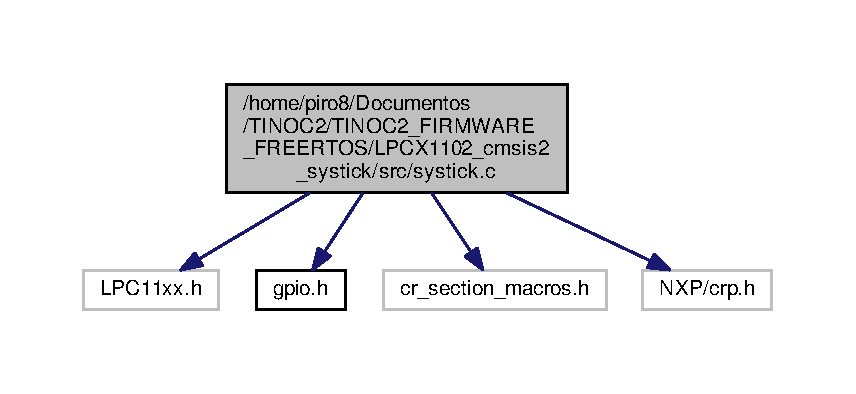
\includegraphics[width=350pt]{systick_8c__incl}
\end{center}
\end{figure}
\subsection*{Macros}
\begin{DoxyCompactItemize}
\item 
\#define \hyperlink{systick_8c_a663daa01e565aee93c6f20c5845b90b4}{L\+E\+D\+\_\+\+P\+O\+RT}~0
\item 
\#define \hyperlink{systick_8c_a59f4211c4d5b67972bfcf5e4c1ba17ca}{L\+E\+D\+\_\+\+B\+IT}~11
\item 
\#define \hyperlink{systick_8c_af2e697ac60e05813d45ea2c9c9e79c25}{L\+E\+D\+\_\+\+ON}~1
\item 
\#define \hyperlink{systick_8c_a80700bb63bd56ebabbb4728aa433fd29}{L\+E\+D\+\_\+\+O\+FF}~0
\item 
\#define \hyperlink{systick_8c_a790fa255763cf3abd5f4c7a693c21462}{D\+E\+L\+A\+Y\+\_\+\+L\+EN}~2000
\end{DoxyCompactItemize}
\subsection*{Functions}
\begin{DoxyCompactItemize}
\item 
void \hyperlink{systick_8c_ab5e09814056d617c521549e542639b7e}{Sys\+Tick\+\_\+\+Handler} (void)
\item 
int \hyperlink{systick_8c_a840291bc02cba5474a4cb46a9b9566fe}{main} (void)
\end{DoxyCompactItemize}
\subsection*{Variables}
\begin{DoxyCompactItemize}
\item 
\+\_\+\+\_\+\+C\+RP const unsigned int \hyperlink{systick_8c_a2cf89d37cd40fb4274f5d428632e9ac5}{C\+R\+P\+\_\+\+W\+O\+RD} = C\+R\+P\+\_\+\+N\+O\+\_\+\+C\+RP
\item 
volatile uint32\+\_\+t \hyperlink{systick_8c_a0a6e5e17fcb15f3922e278025acabfa2}{ms\+Ticks}
\end{DoxyCompactItemize}


\subsection{Macro Definition Documentation}
\index{systick.\+c@{systick.\+c}!D\+E\+L\+A\+Y\+\_\+\+L\+EN@{D\+E\+L\+A\+Y\+\_\+\+L\+EN}}
\index{D\+E\+L\+A\+Y\+\_\+\+L\+EN@{D\+E\+L\+A\+Y\+\_\+\+L\+EN}!systick.\+c@{systick.\+c}}
\subsubsection[{\texorpdfstring{D\+E\+L\+A\+Y\+\_\+\+L\+EN}{DELAY_LEN}}]{\setlength{\rightskip}{0pt plus 5cm}\#define D\+E\+L\+A\+Y\+\_\+\+L\+EN~2000}\hypertarget{systick_8c_a790fa255763cf3abd5f4c7a693c21462}{}\label{systick_8c_a790fa255763cf3abd5f4c7a693c21462}


Definition at line 62 of file systick.\+c.

\index{systick.\+c@{systick.\+c}!L\+E\+D\+\_\+\+B\+IT@{L\+E\+D\+\_\+\+B\+IT}}
\index{L\+E\+D\+\_\+\+B\+IT@{L\+E\+D\+\_\+\+B\+IT}!systick.\+c@{systick.\+c}}
\subsubsection[{\texorpdfstring{L\+E\+D\+\_\+\+B\+IT}{LED_BIT}}]{\setlength{\rightskip}{0pt plus 5cm}\#define L\+E\+D\+\_\+\+B\+IT~11}\hypertarget{systick_8c_a59f4211c4d5b67972bfcf5e4c1ba17ca}{}\label{systick_8c_a59f4211c4d5b67972bfcf5e4c1ba17ca}


Definition at line 57 of file systick.\+c.

\index{systick.\+c@{systick.\+c}!L\+E\+D\+\_\+\+O\+FF@{L\+E\+D\+\_\+\+O\+FF}}
\index{L\+E\+D\+\_\+\+O\+FF@{L\+E\+D\+\_\+\+O\+FF}!systick.\+c@{systick.\+c}}
\subsubsection[{\texorpdfstring{L\+E\+D\+\_\+\+O\+FF}{LED_OFF}}]{\setlength{\rightskip}{0pt plus 5cm}\#define L\+E\+D\+\_\+\+O\+FF~0}\hypertarget{systick_8c_a80700bb63bd56ebabbb4728aa433fd29}{}\label{systick_8c_a80700bb63bd56ebabbb4728aa433fd29}


Definition at line 59 of file systick.\+c.

\index{systick.\+c@{systick.\+c}!L\+E\+D\+\_\+\+ON@{L\+E\+D\+\_\+\+ON}}
\index{L\+E\+D\+\_\+\+ON@{L\+E\+D\+\_\+\+ON}!systick.\+c@{systick.\+c}}
\subsubsection[{\texorpdfstring{L\+E\+D\+\_\+\+ON}{LED_ON}}]{\setlength{\rightskip}{0pt plus 5cm}\#define L\+E\+D\+\_\+\+ON~1}\hypertarget{systick_8c_af2e697ac60e05813d45ea2c9c9e79c25}{}\label{systick_8c_af2e697ac60e05813d45ea2c9c9e79c25}


Definition at line 58 of file systick.\+c.

\index{systick.\+c@{systick.\+c}!L\+E\+D\+\_\+\+P\+O\+RT@{L\+E\+D\+\_\+\+P\+O\+RT}}
\index{L\+E\+D\+\_\+\+P\+O\+RT@{L\+E\+D\+\_\+\+P\+O\+RT}!systick.\+c@{systick.\+c}}
\subsubsection[{\texorpdfstring{L\+E\+D\+\_\+\+P\+O\+RT}{LED_PORT}}]{\setlength{\rightskip}{0pt plus 5cm}\#define L\+E\+D\+\_\+\+P\+O\+RT~0}\hypertarget{systick_8c_a663daa01e565aee93c6f20c5845b90b4}{}\label{systick_8c_a663daa01e565aee93c6f20c5845b90b4}


Definition at line 56 of file systick.\+c.



\subsection{Function Documentation}
\index{systick.\+c@{systick.\+c}!main@{main}}
\index{main@{main}!systick.\+c@{systick.\+c}}
\subsubsection[{\texorpdfstring{main(void)}{main(void)}}]{\setlength{\rightskip}{0pt plus 5cm}int main (
\begin{DoxyParamCaption}
\item[{void}]{}
\end{DoxyParamCaption}
)}\hypertarget{systick_8c_a840291bc02cba5474a4cb46a9b9566fe}{}\label{systick_8c_a840291bc02cba5474a4cb46a9b9566fe}


Definition at line 84 of file systick.\+c.

\index{systick.\+c@{systick.\+c}!Sys\+Tick\+\_\+\+Handler@{Sys\+Tick\+\_\+\+Handler}}
\index{Sys\+Tick\+\_\+\+Handler@{Sys\+Tick\+\_\+\+Handler}!systick.\+c@{systick.\+c}}
\subsubsection[{\texorpdfstring{Sys\+Tick\+\_\+\+Handler(void)}{SysTick_Handler(void)}}]{\setlength{\rightskip}{0pt plus 5cm}void Sys\+Tick\+\_\+\+Handler (
\begin{DoxyParamCaption}
\item[{void}]{}
\end{DoxyParamCaption}
)}\hypertarget{systick_8c_ab5e09814056d617c521549e542639b7e}{}\label{systick_8c_ab5e09814056d617c521549e542639b7e}


Definition at line 68 of file systick.\+c.



\subsection{Variable Documentation}
\index{systick.\+c@{systick.\+c}!C\+R\+P\+\_\+\+W\+O\+RD@{C\+R\+P\+\_\+\+W\+O\+RD}}
\index{C\+R\+P\+\_\+\+W\+O\+RD@{C\+R\+P\+\_\+\+W\+O\+RD}!systick.\+c@{systick.\+c}}
\subsubsection[{\texorpdfstring{C\+R\+P\+\_\+\+W\+O\+RD}{CRP_WORD}}]{\setlength{\rightskip}{0pt plus 5cm}\+\_\+\+\_\+\+C\+RP const unsigned int C\+R\+P\+\_\+\+W\+O\+RD = C\+R\+P\+\_\+\+N\+O\+\_\+\+C\+RP}\hypertarget{systick_8c_a2cf89d37cd40fb4274f5d428632e9ac5}{}\label{systick_8c_a2cf89d37cd40fb4274f5d428632e9ac5}


Definition at line 52 of file systick.\+c.

\index{systick.\+c@{systick.\+c}!ms\+Ticks@{ms\+Ticks}}
\index{ms\+Ticks@{ms\+Ticks}!systick.\+c@{systick.\+c}}
\subsubsection[{\texorpdfstring{ms\+Ticks}{msTicks}}]{\setlength{\rightskip}{0pt plus 5cm}volatile uint32\+\_\+t ms\+Ticks}\hypertarget{systick_8c_a0a6e5e17fcb15f3922e278025acabfa2}{}\label{systick_8c_a0a6e5e17fcb15f3922e278025acabfa2}


Definition at line 64 of file systick.\+c.


%--- End generated contents ---

% Index
\backmatter
\newpage
\phantomsection
\clearemptydoublepage
\addcontentsline{toc}{chapter}{Index}
\printindex

\end{document}
